% Use only LaTeX2e, calling the article.cls class and 12-point type.

\documentclass[11pt]{article}

% Users of the {thebibliography} environment or BibTeX should use the
% scicite.sty package, downloadable from *Science* at
% www.sciencemag.org/about/authors/prep/TeX_help/ .
% This package should properly format in-text
% reference calls and reference-list numbers.

%\usepackage{scicite}

% Use times if you have the font installed; otherwise, comment out the
% following line.

\usepackage{times}
\usepackage{setspace}
\usepackage{threeparttable}
\usepackage{caption}
\usepackage{subcaption}
\usepackage{graphicx}
\usepackage{hyperref}
\usepackage{placeins}
\usepackage{multirow}
\usepackage[english]{babel}
\usepackage{natbib}
\bibliographystyle{abbrvnat}
\setcitestyle{authoryear,round} %Citation-related commands

% The preamble here sets up a lot of new/revised commands and
% environments.  It's annoying, but please do *not* try to strip these
% out into a separate .sty file (which could lead to the loss of some
% information when we convert the file to other formats).  Instead, keep
% them in the preamble of your main LaTeX source file.


% The following parameters seem to provide a reasonable page setup.

\topmargin 0.0cm
\oddsidemargin 0.2cm
\textwidth 16cm 
\textheight 21cm
\footskip 1.0cm


%The next command sets up an environment for the abstract to your paper.

\newenvironment{sciabstract}{%
	\begin{quote} \bf}
	{\end{quote}}


% If your reference list includes text notes as well as references,
% include the following line; otherwise, comment it out.
\newcommand\fnote[1]{\captionsetup{font=small}\caption*{#1}}
\renewcommand\refname{References and Notes}

% The following lines set up an environment for the last note in the
% reference list, which commonly includes acknowledgments of funding,
% help, etc.  It's intended for users of BibTeX or the {thebibliography}
% environment.  Users who are hand-coding their references at the end
% using a list environment such as {enumerate} can simply add another
% item at the end, and it will be numbered automatically.

\newcounter{lastnote}
\newenvironment{scilastnote}{%
	\setcounter{lastnote}{\value{enumiv}}%
	\addtocounter{lastnote}{+1}%
	\begin{list}%
		{\arabic{lastnote}.}
		{\setlength{\leftmargin}{.22in}}
		{\setlength{\labelsep}{.5em}}}
	{\end{list}}


% Include your paper's title here

\title{\textbf{NeuroFlow Data Task}\\
	--- Main Report --}

\author{Tao Song}

\begin{document} 
	
	% Double-space the manuscript.
	
\baselineskip24pt
	
	% Make the title.
\maketitle 
	% Place your abstract within the special {sciabstract} environment.
	
	
\renewcommand{\abstractname}{Introduction}
\begin{abstract}
	This report starts by providing a directory of files uploaded in the github repo. In the main body of the report, I provided detailed information of examinations and analysis I conducted in better understanding the dataset and providing potential solutions. 
	I began with manipulating the dataset and conducting some exploratory analysis. These includes: slicing and reshaping the dataset with generating add potentially interesting variables, exploring the distributions (patterns) of several key variables both across the whole dataaset and limited to a defined target patient group (patients whose first-visit anxiety score equals to or is larger than 10). I then conducted some exploratory analysis, such as regression analysis (linear and logistic) as well as some other interesting comparisons. Lastly, I discussed what information might be interesting or potentially useful to collect and added some interesting tests in exploring the effect potentially exerted by control variables. 
\end{abstract}
	
\singlespacing
\tableofcontents
	
\newpage
	
\section{Github repo directory}
	
Here is a detailed list of files and their brief information:
\begin{itemize}
	\item \textbf{Foler data\_task:} the main code, in R;
	\item \textbf{Figures:} all figures produced in exploration;
	\item \textbf{phq\_all\_long\_format.csv:} the long-formated dataset with additional variables;
	\item \textbf{phq\_all\_wide\_format.csv:} the wide-formated dataset with additional variables;
	\item \textbf{report.tex:} the latex script in generating the main report;
	\item \textbf{report.pdf:} the main report;
	\item \textbf{The rest 2 files are the original task description and dataset.}
\end{itemize}

\section{Data manipulation and distribution}

After going through the task description and the dataset carefully, I firstly added some variables for the purpose of further analysis. The first (test date) and the third column (patient-record-creating date) produced 3 more variables that describe "year-month-day", "hour-minute-second", and "am / pm" separately. Variable "number\_of\_visits" is added for each patient in indicating the number of visits each patient made. Later in Section \ref{ss:sec2}, a dichotomous variable "improve" is added and used as the outcome variable such that it gets 1 if the anxiety score in the last-visit is lower than the score in this patient's first-visit. Worth noticing that there is one patient (with patient\_id 10687) standing out with over 80 clinical visits. This patient had an extremely high visiting frequency of almost testing every other day. I excluded this particular patient because he/she is clearly an outlier that needs separate consideration.

Firstly, I want to have a better understanding of what the dataset entails. Among 53,698 patient records in the full dataset, there are in total 15,501 unique patients. Figure \ref{fig:picture1} presents the density plots for 3 key variables: the number of visits, anxiety score on the first-visit, anxiety score on the last-visit. The red vertical line indicates the mode and the blue line is the mean. We can see that most patients in this dataset only visited and measured their anxiety once as presented in plot (a). The average visiting frequency is around three or four times. The average anxiety score of patients on the first-visit is 5.5, the average for the last-visit is 4.9. The boxplot in plot (d) presents the comparison between scores on the first-visit versus last-visit in a more straightforward manner. Although we can observe a descrease of anxiety on average by these plots, it's simply a very broad and crude exploration. Let's further investigate more details with multiple dimensions.

\begin{figure}[htb!]
	\caption{Density plots: the full dataset}\label{fig:picture1}
	\begin{subfigure}[h]{0.48\linewidth}
		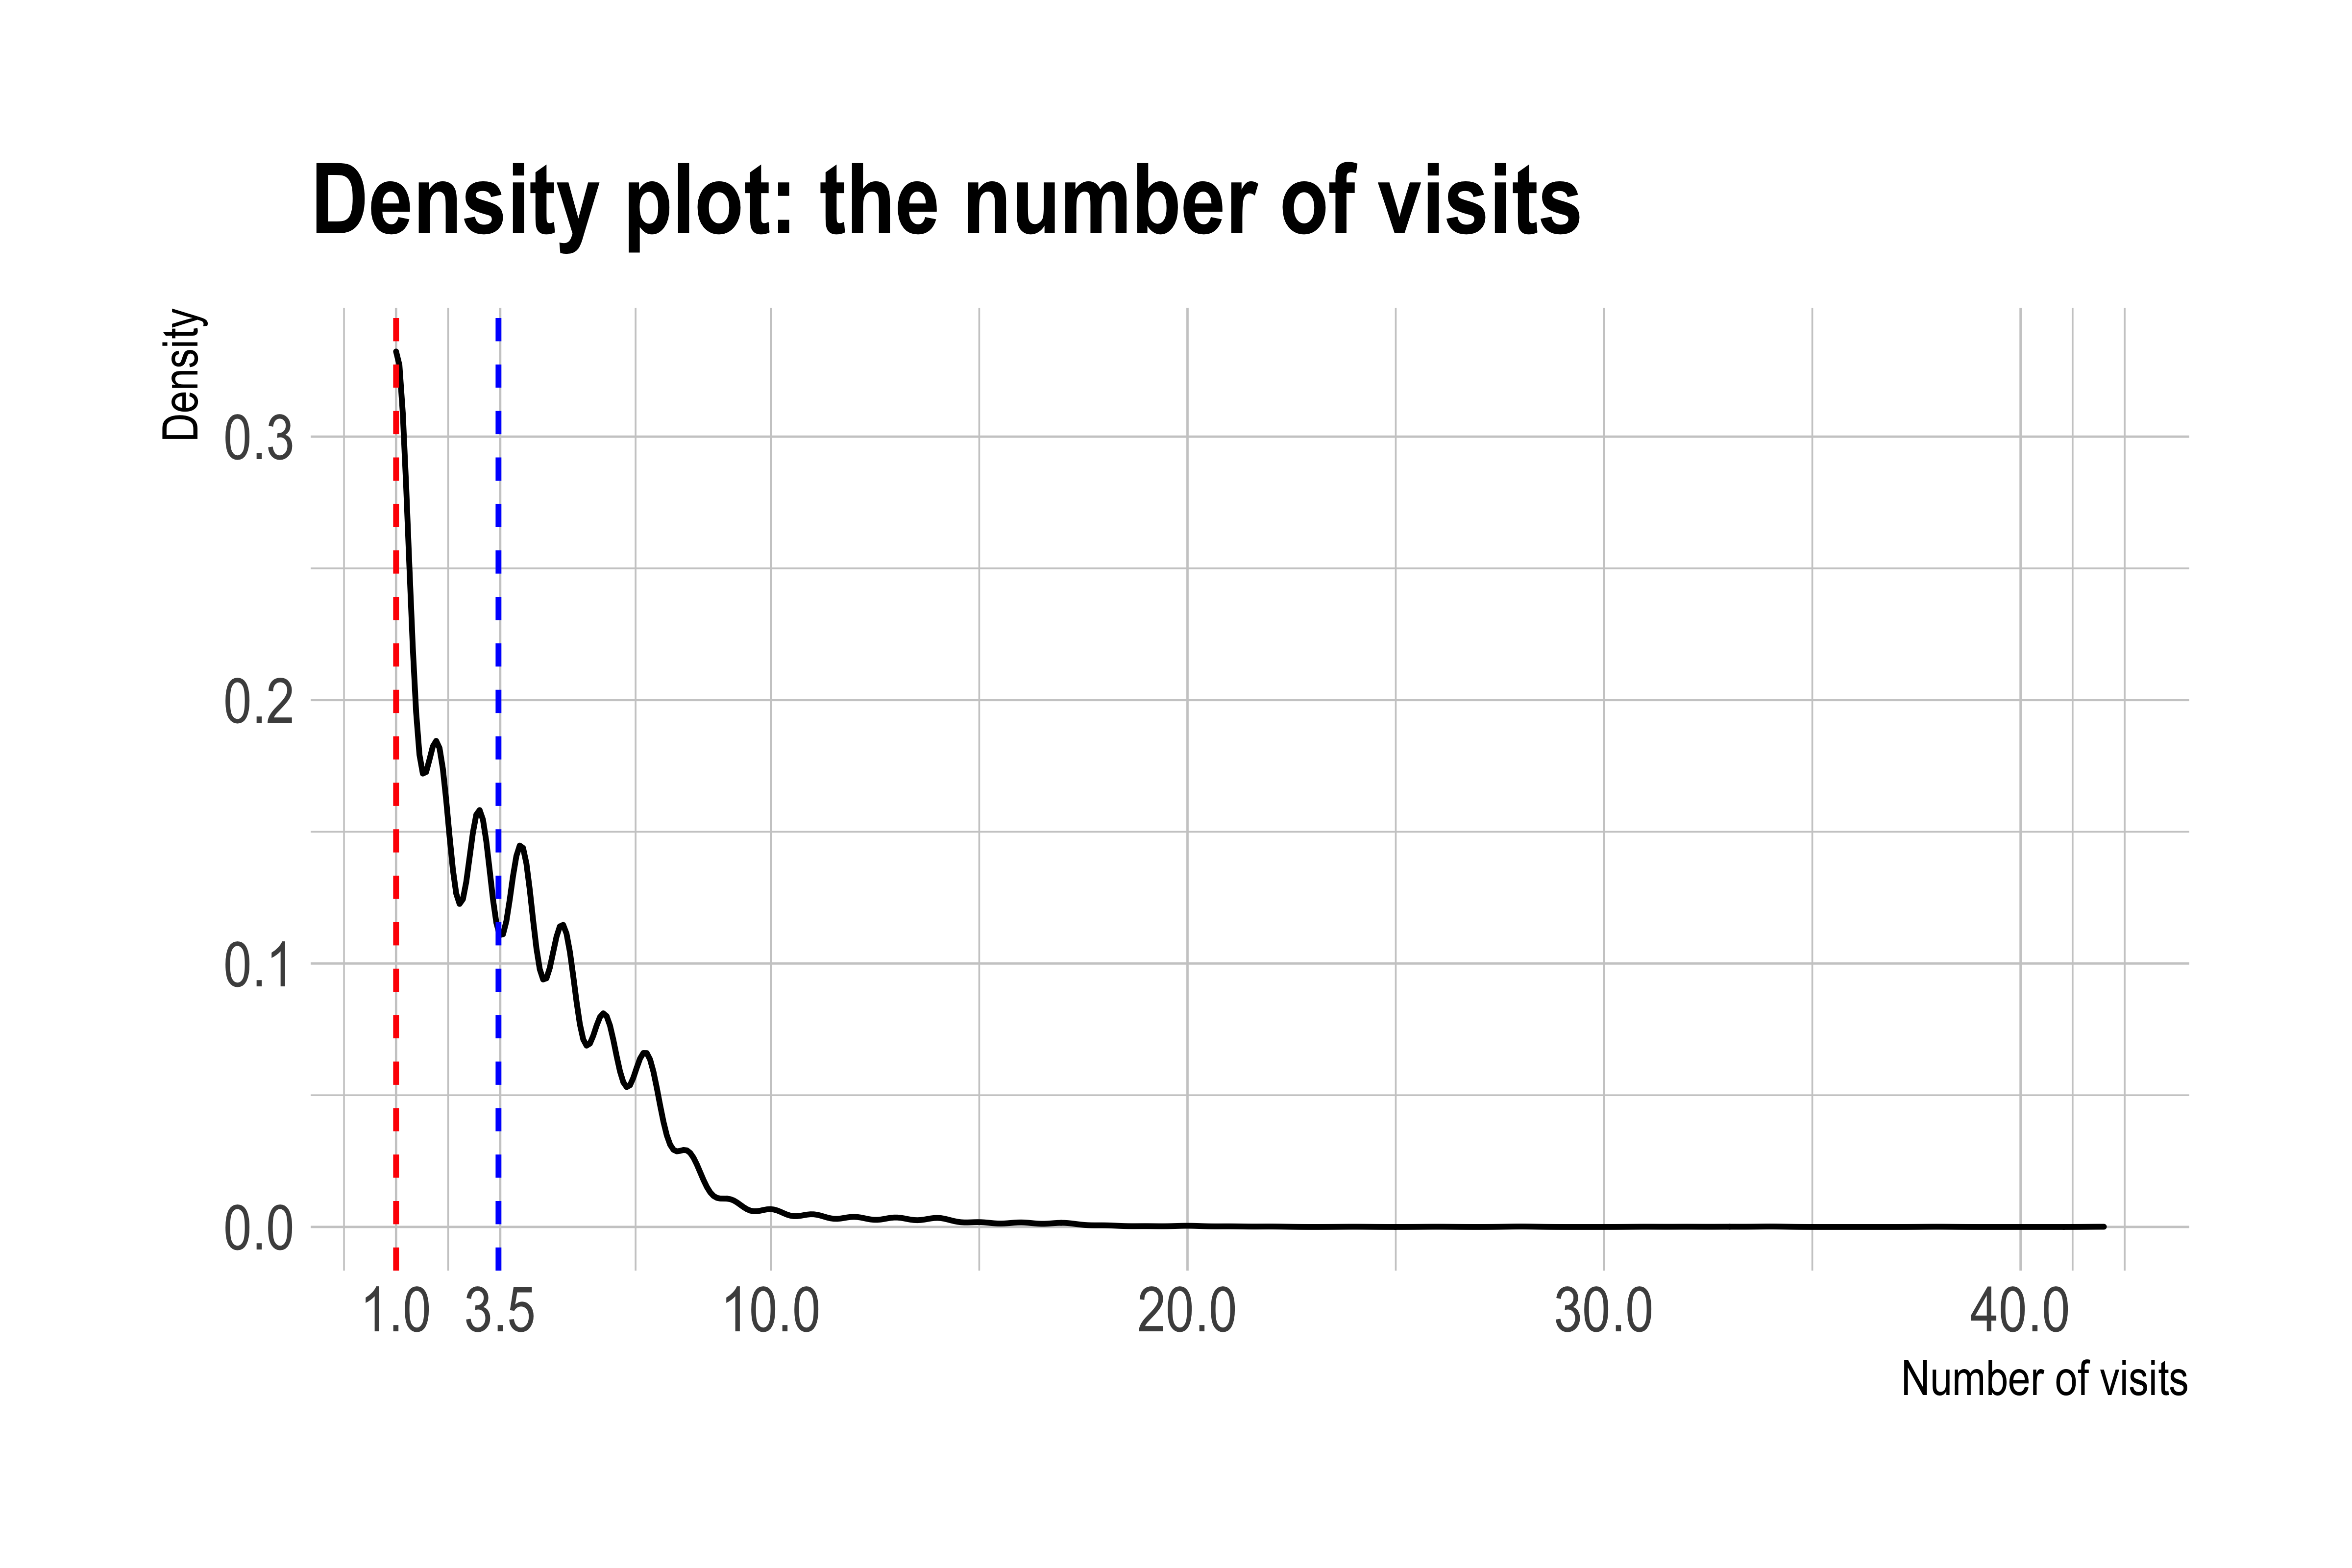
\includegraphics[width=\linewidth]{Figures/p1.png}
		\caption{}\label{fig:p1}
	\end{subfigure}
	\hfill
	\begin{subfigure}[h]{0.48\linewidth}
		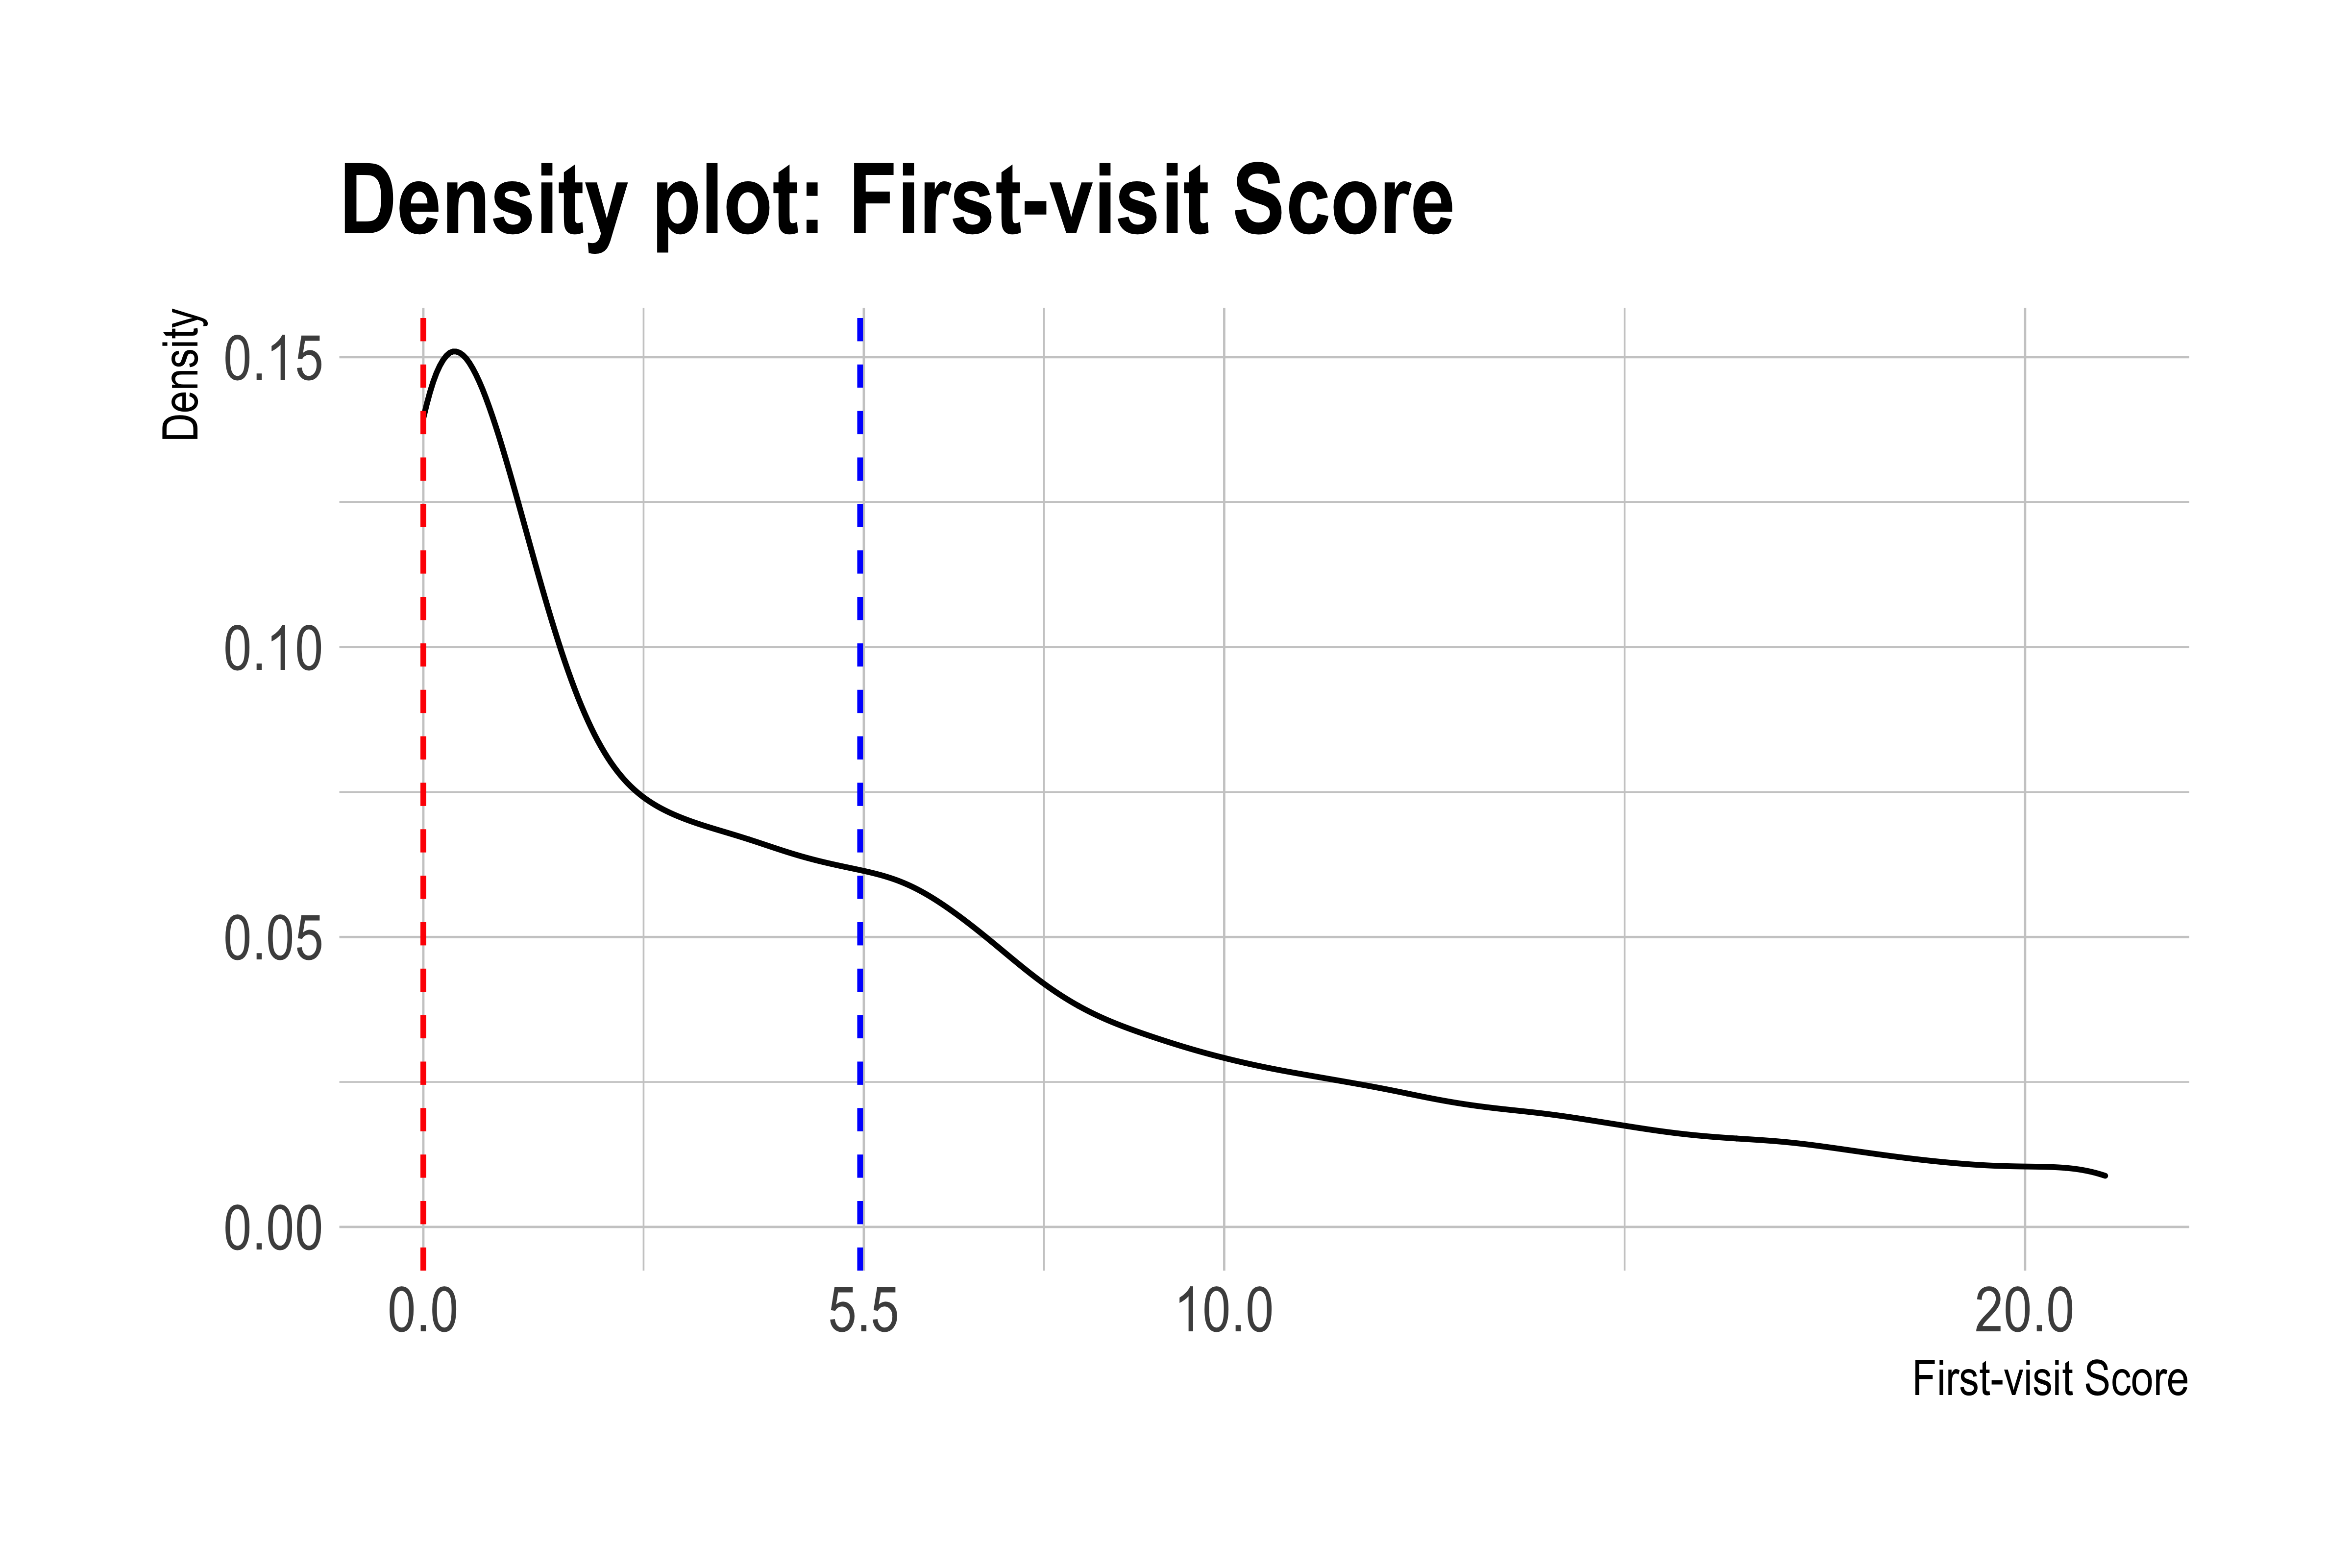
\includegraphics[width=\linewidth]{Figures/p2.png}
		\caption{}\label{fig:p2}
	\end{subfigure}
	\hfill
	\begin{subfigure}[h]{0.48\linewidth}
		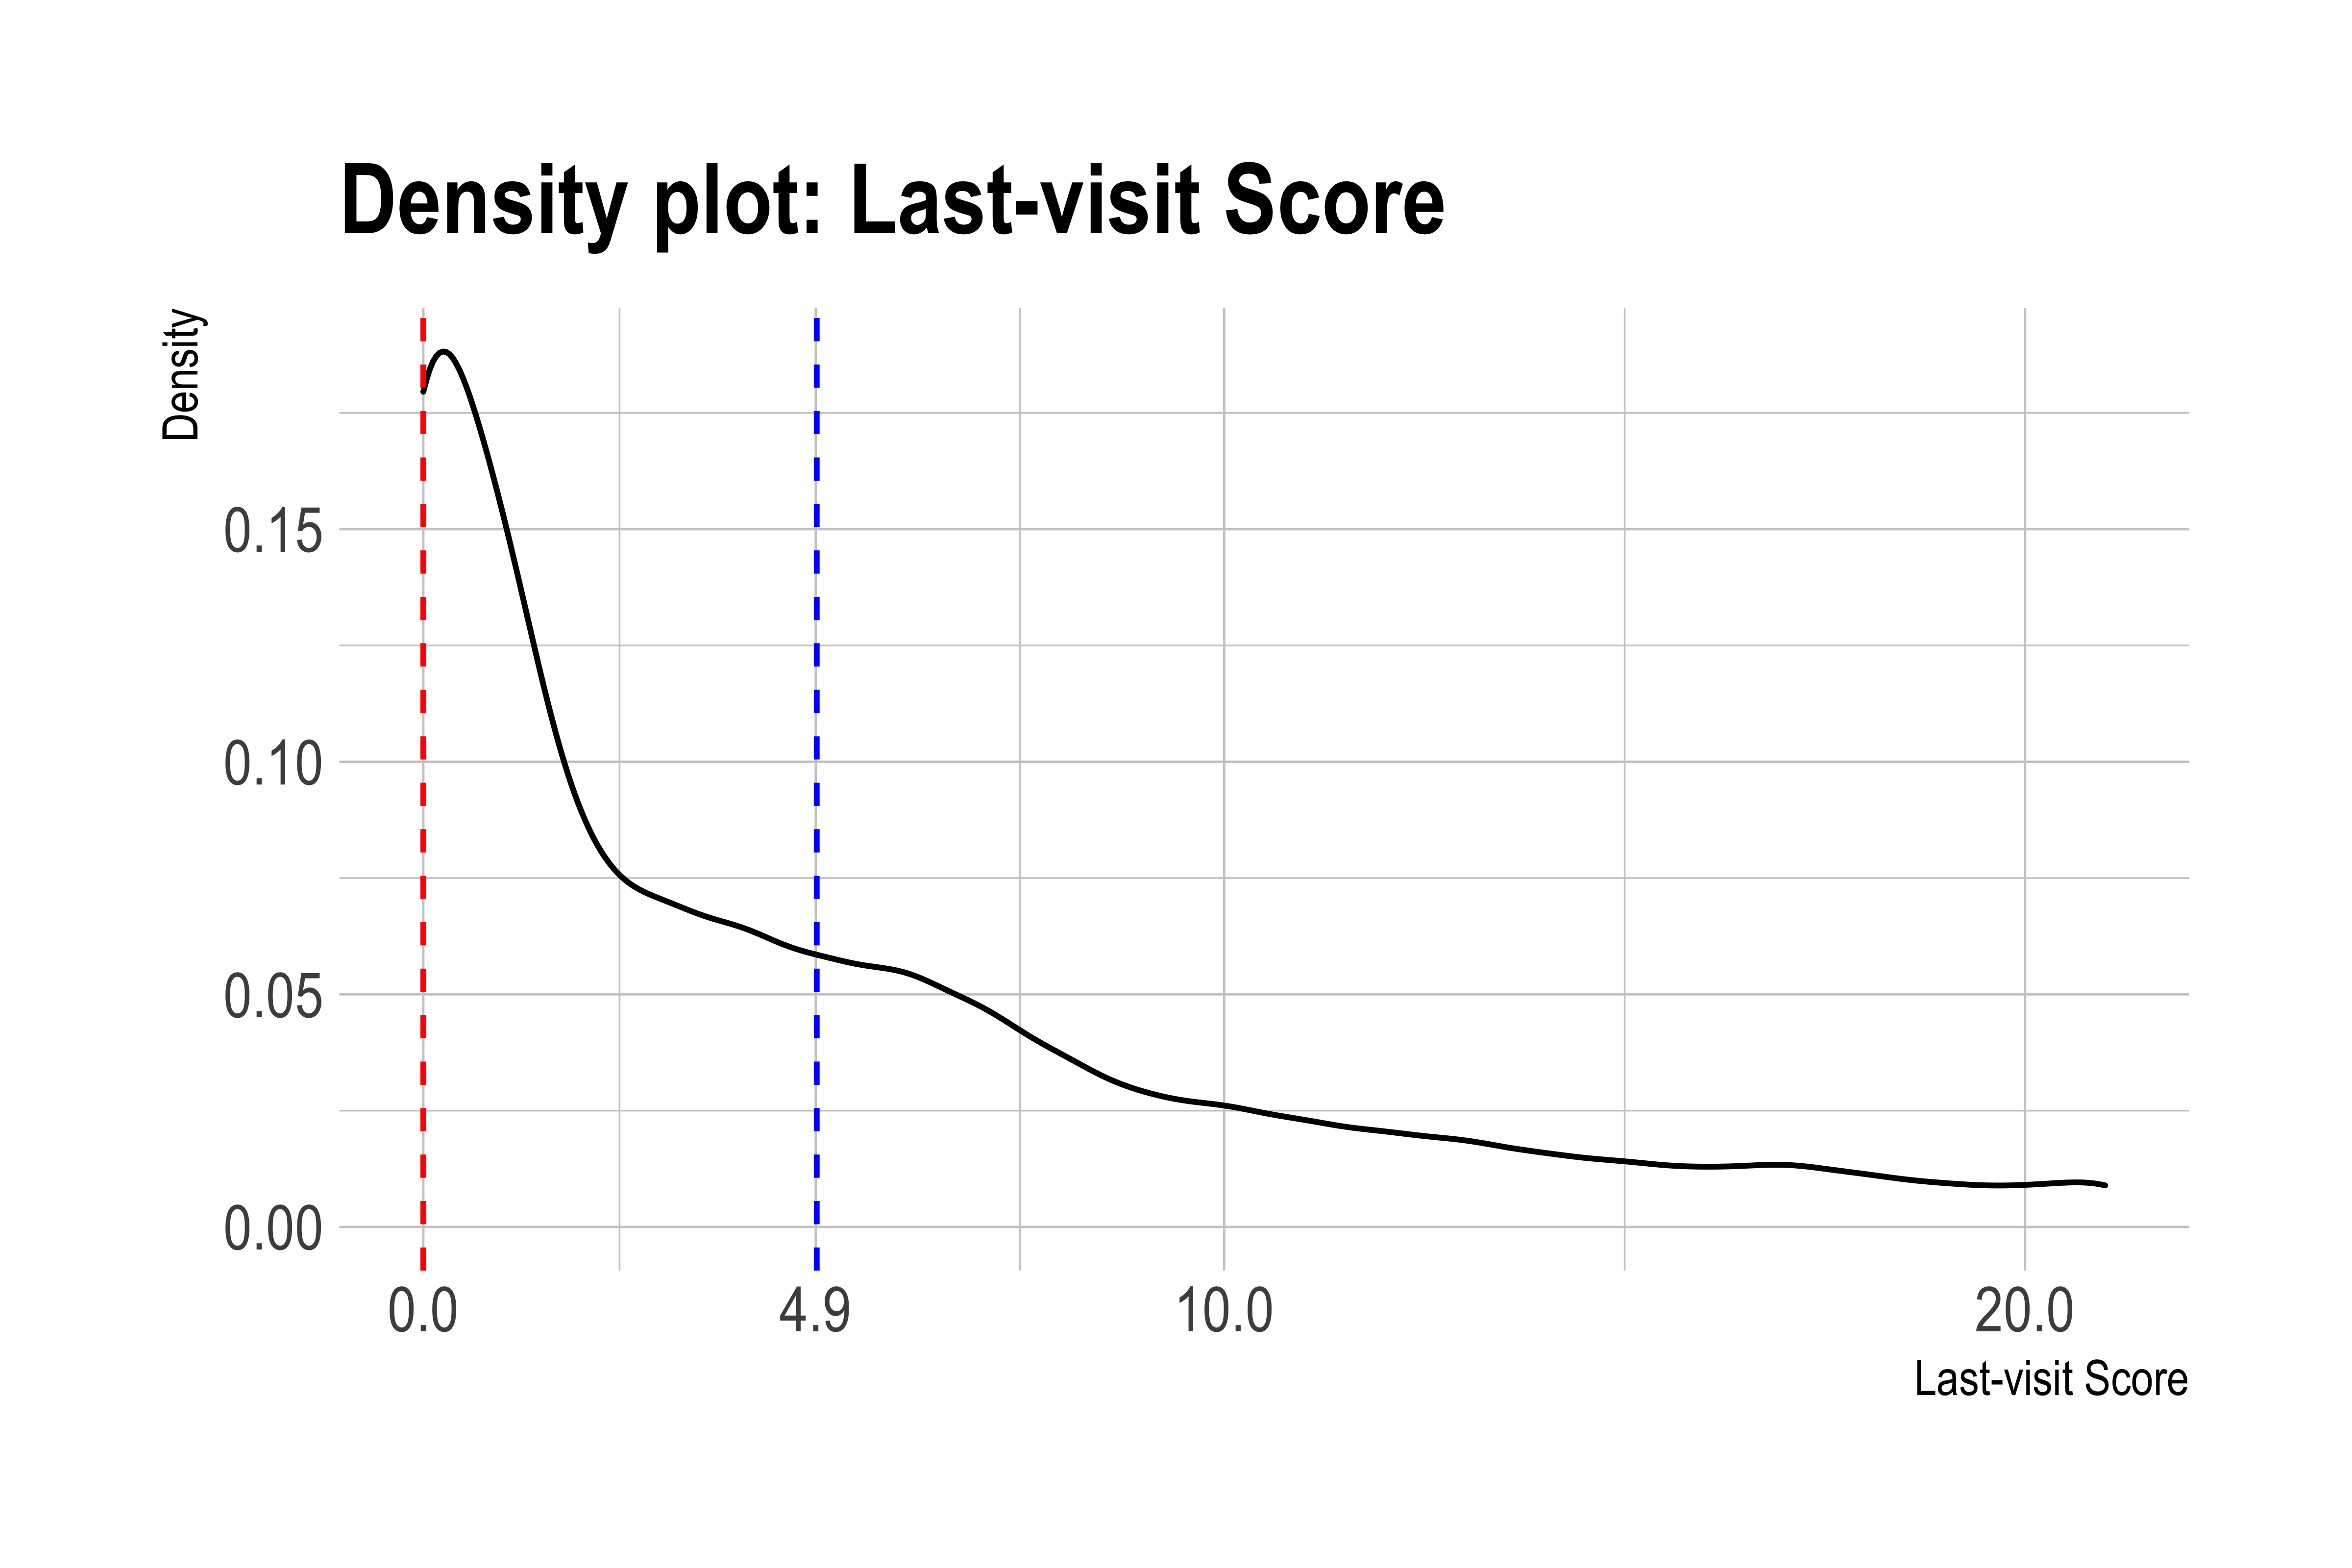
\includegraphics[width=\linewidth]{Figures/p3.png}
		\caption{}\label{fig:p3}
	\end{subfigure}
	\hfill
	\begin{subfigure}[h]{0.48\linewidth}
	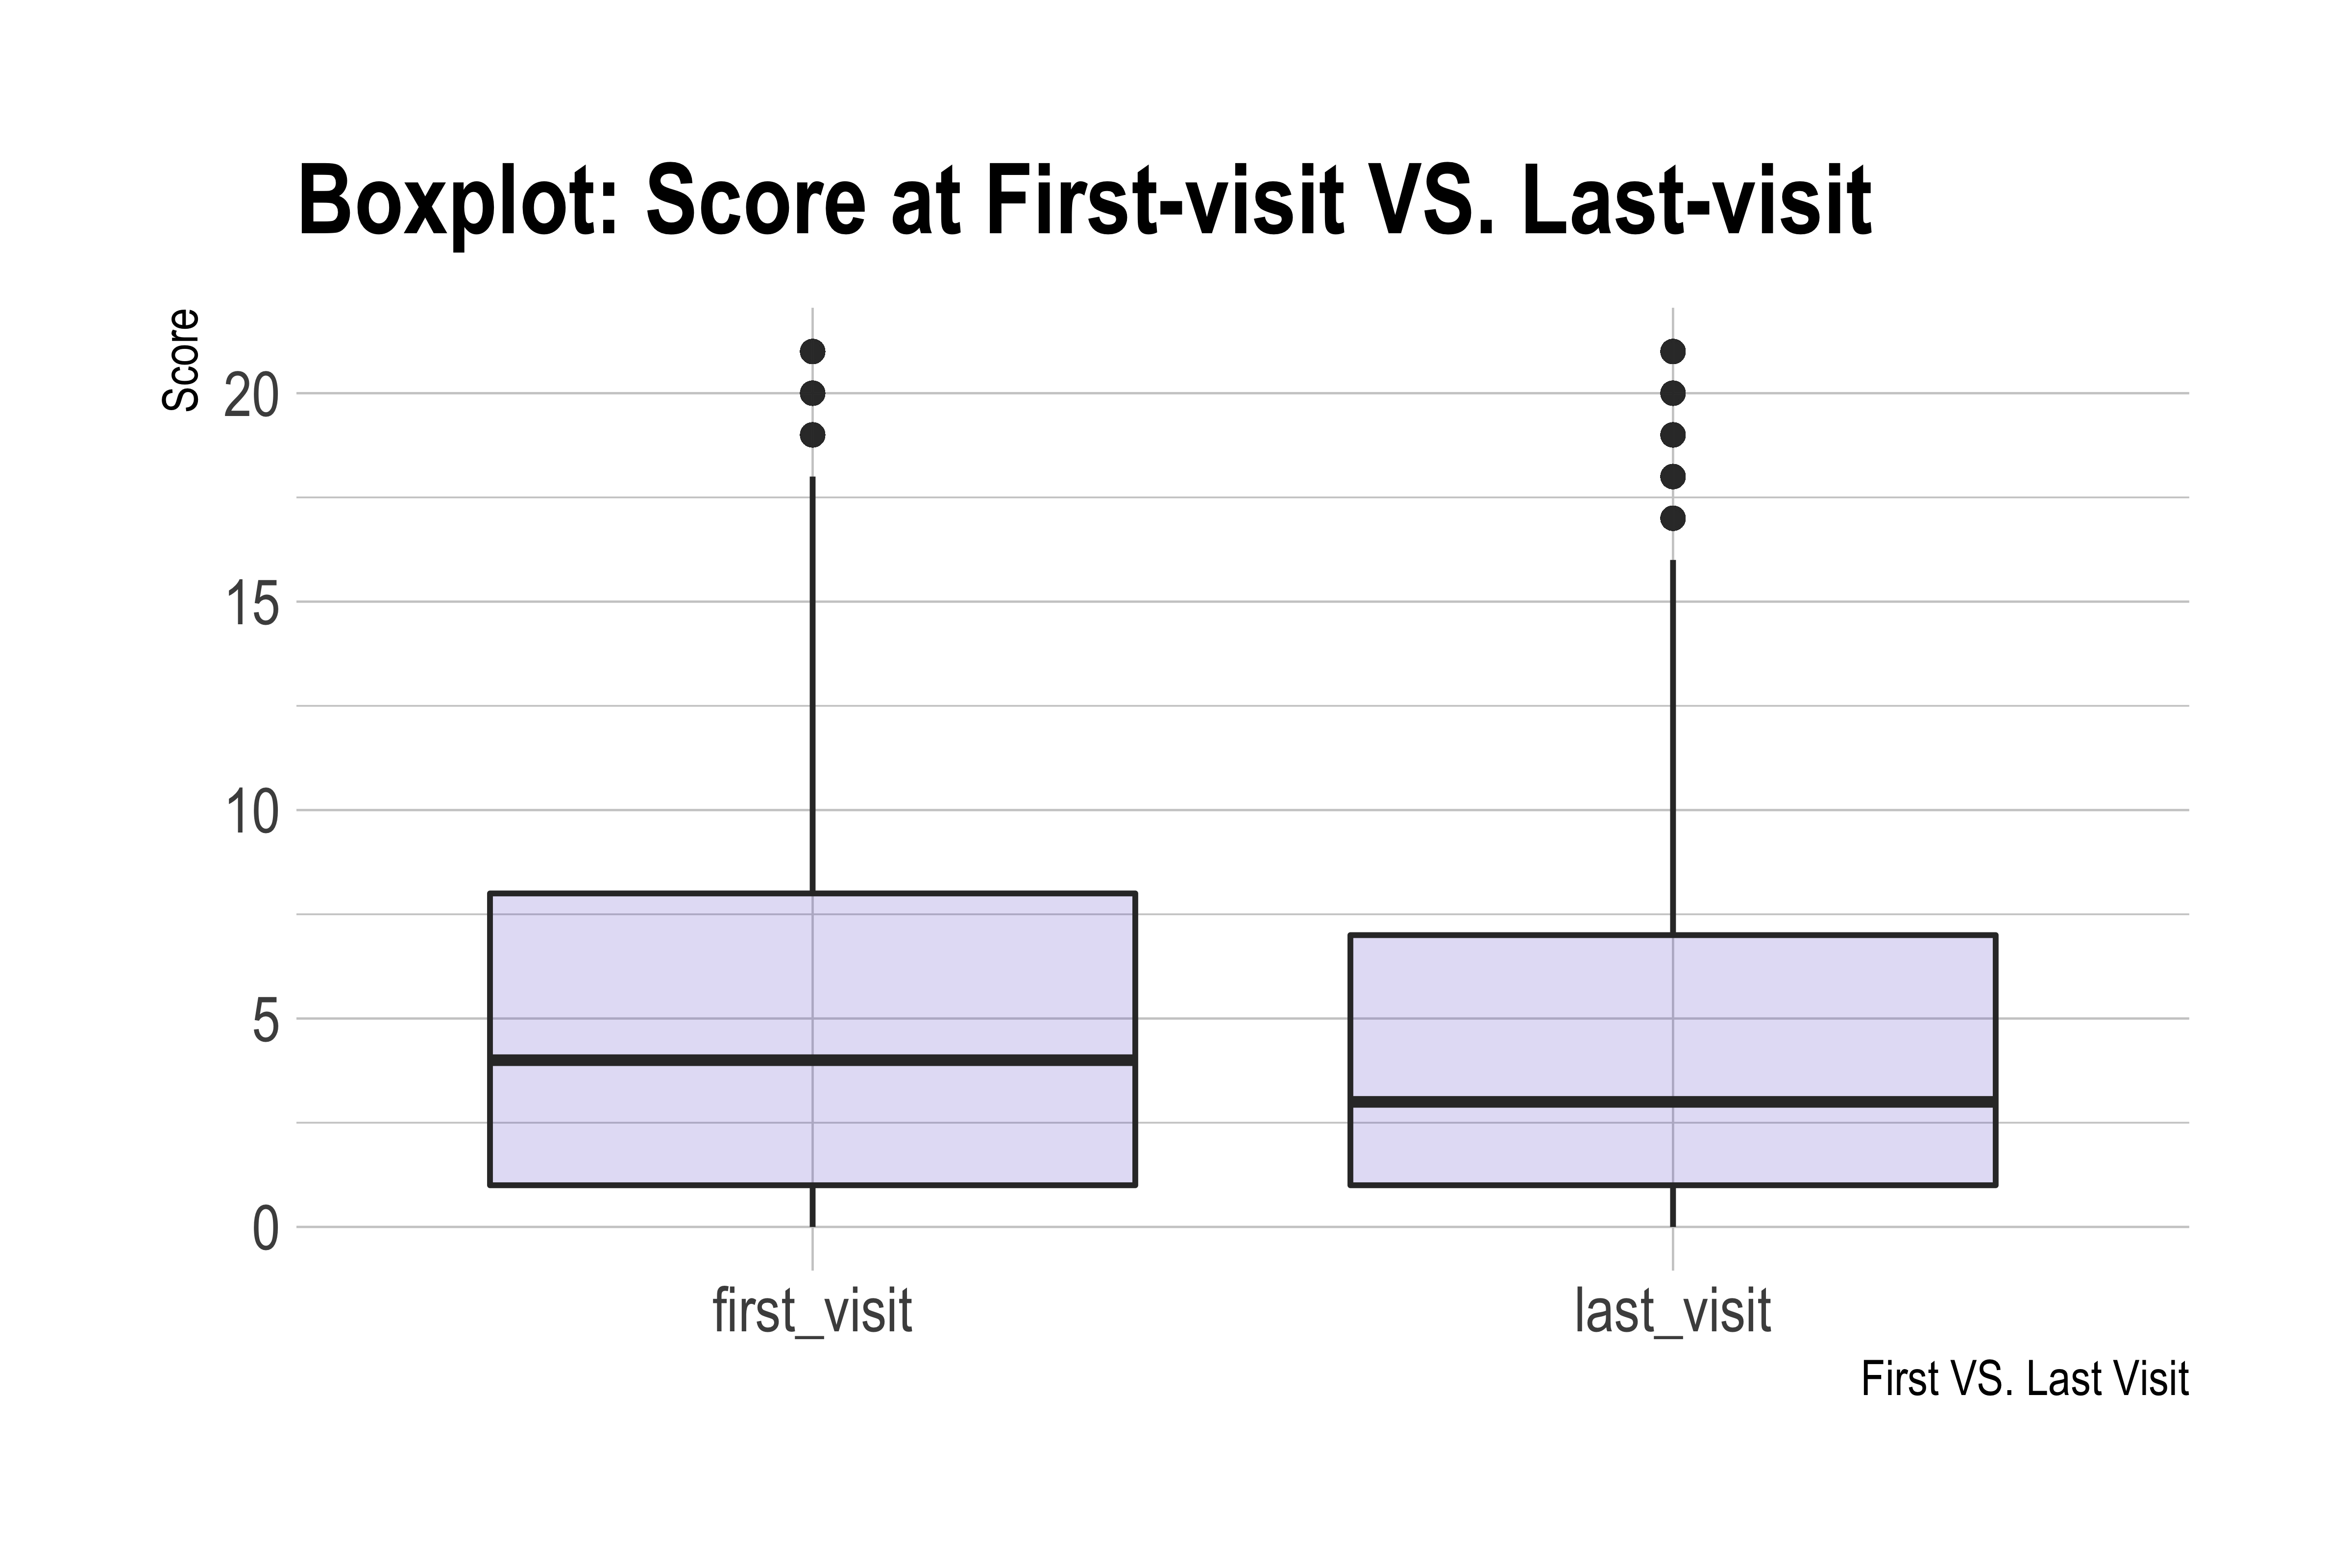
\includegraphics[width=\linewidth]{Figures/p4.png}
	\caption{}\label{fig:p4}
	\end{subfigure}
\end{figure}

The full list of patients should clearly not be our focus of interests. One key process is to define the target patients and subset our dataset. The targeting patients should provide enough information for us to analyse and make potential observations. Our ultimate objective is to better visualize the process which enbodies both the assessment as a measure and the ongoing clinical treatment for some patients so that both mental health providers and patients have a more intuitive understanding of the potential treatment effect. Patients who do not need further clinical evaluation (have an anxiety score less than 10) would hardly provide valuable information on whether patients' anxiety could be released by clinical help. Also, patients who pay very few visits are also providing quite limited information because too many factors might come into play and we do not have the statistical power in making any plausible conclusion. 

Figure \ref{fig:picture2} presents some interesting trends. From the quite similar density plot of visiting-frequency, patients with higher initial anxiety levels in our datasets did not pay more visits as we might have imagined. Also, plot (c) shows a mixed pattern such that some patients indeed lowered their anxiety at last while we also still see many that did not. But we can see that the variation within this specific targeting group is smaller for both first-vist score and last-visit score. Also the mean of last-visit score decreased more compared to the plot (d) in figure \ref{fig:picture1}.

 \begin{figure}[htb!]
 	\caption{Density plots: subset to patients who has anxiety score equals to or larger than 10}\label{fig:picture2}
 	\begin{subfigure}[h]{0.48\linewidth}
 		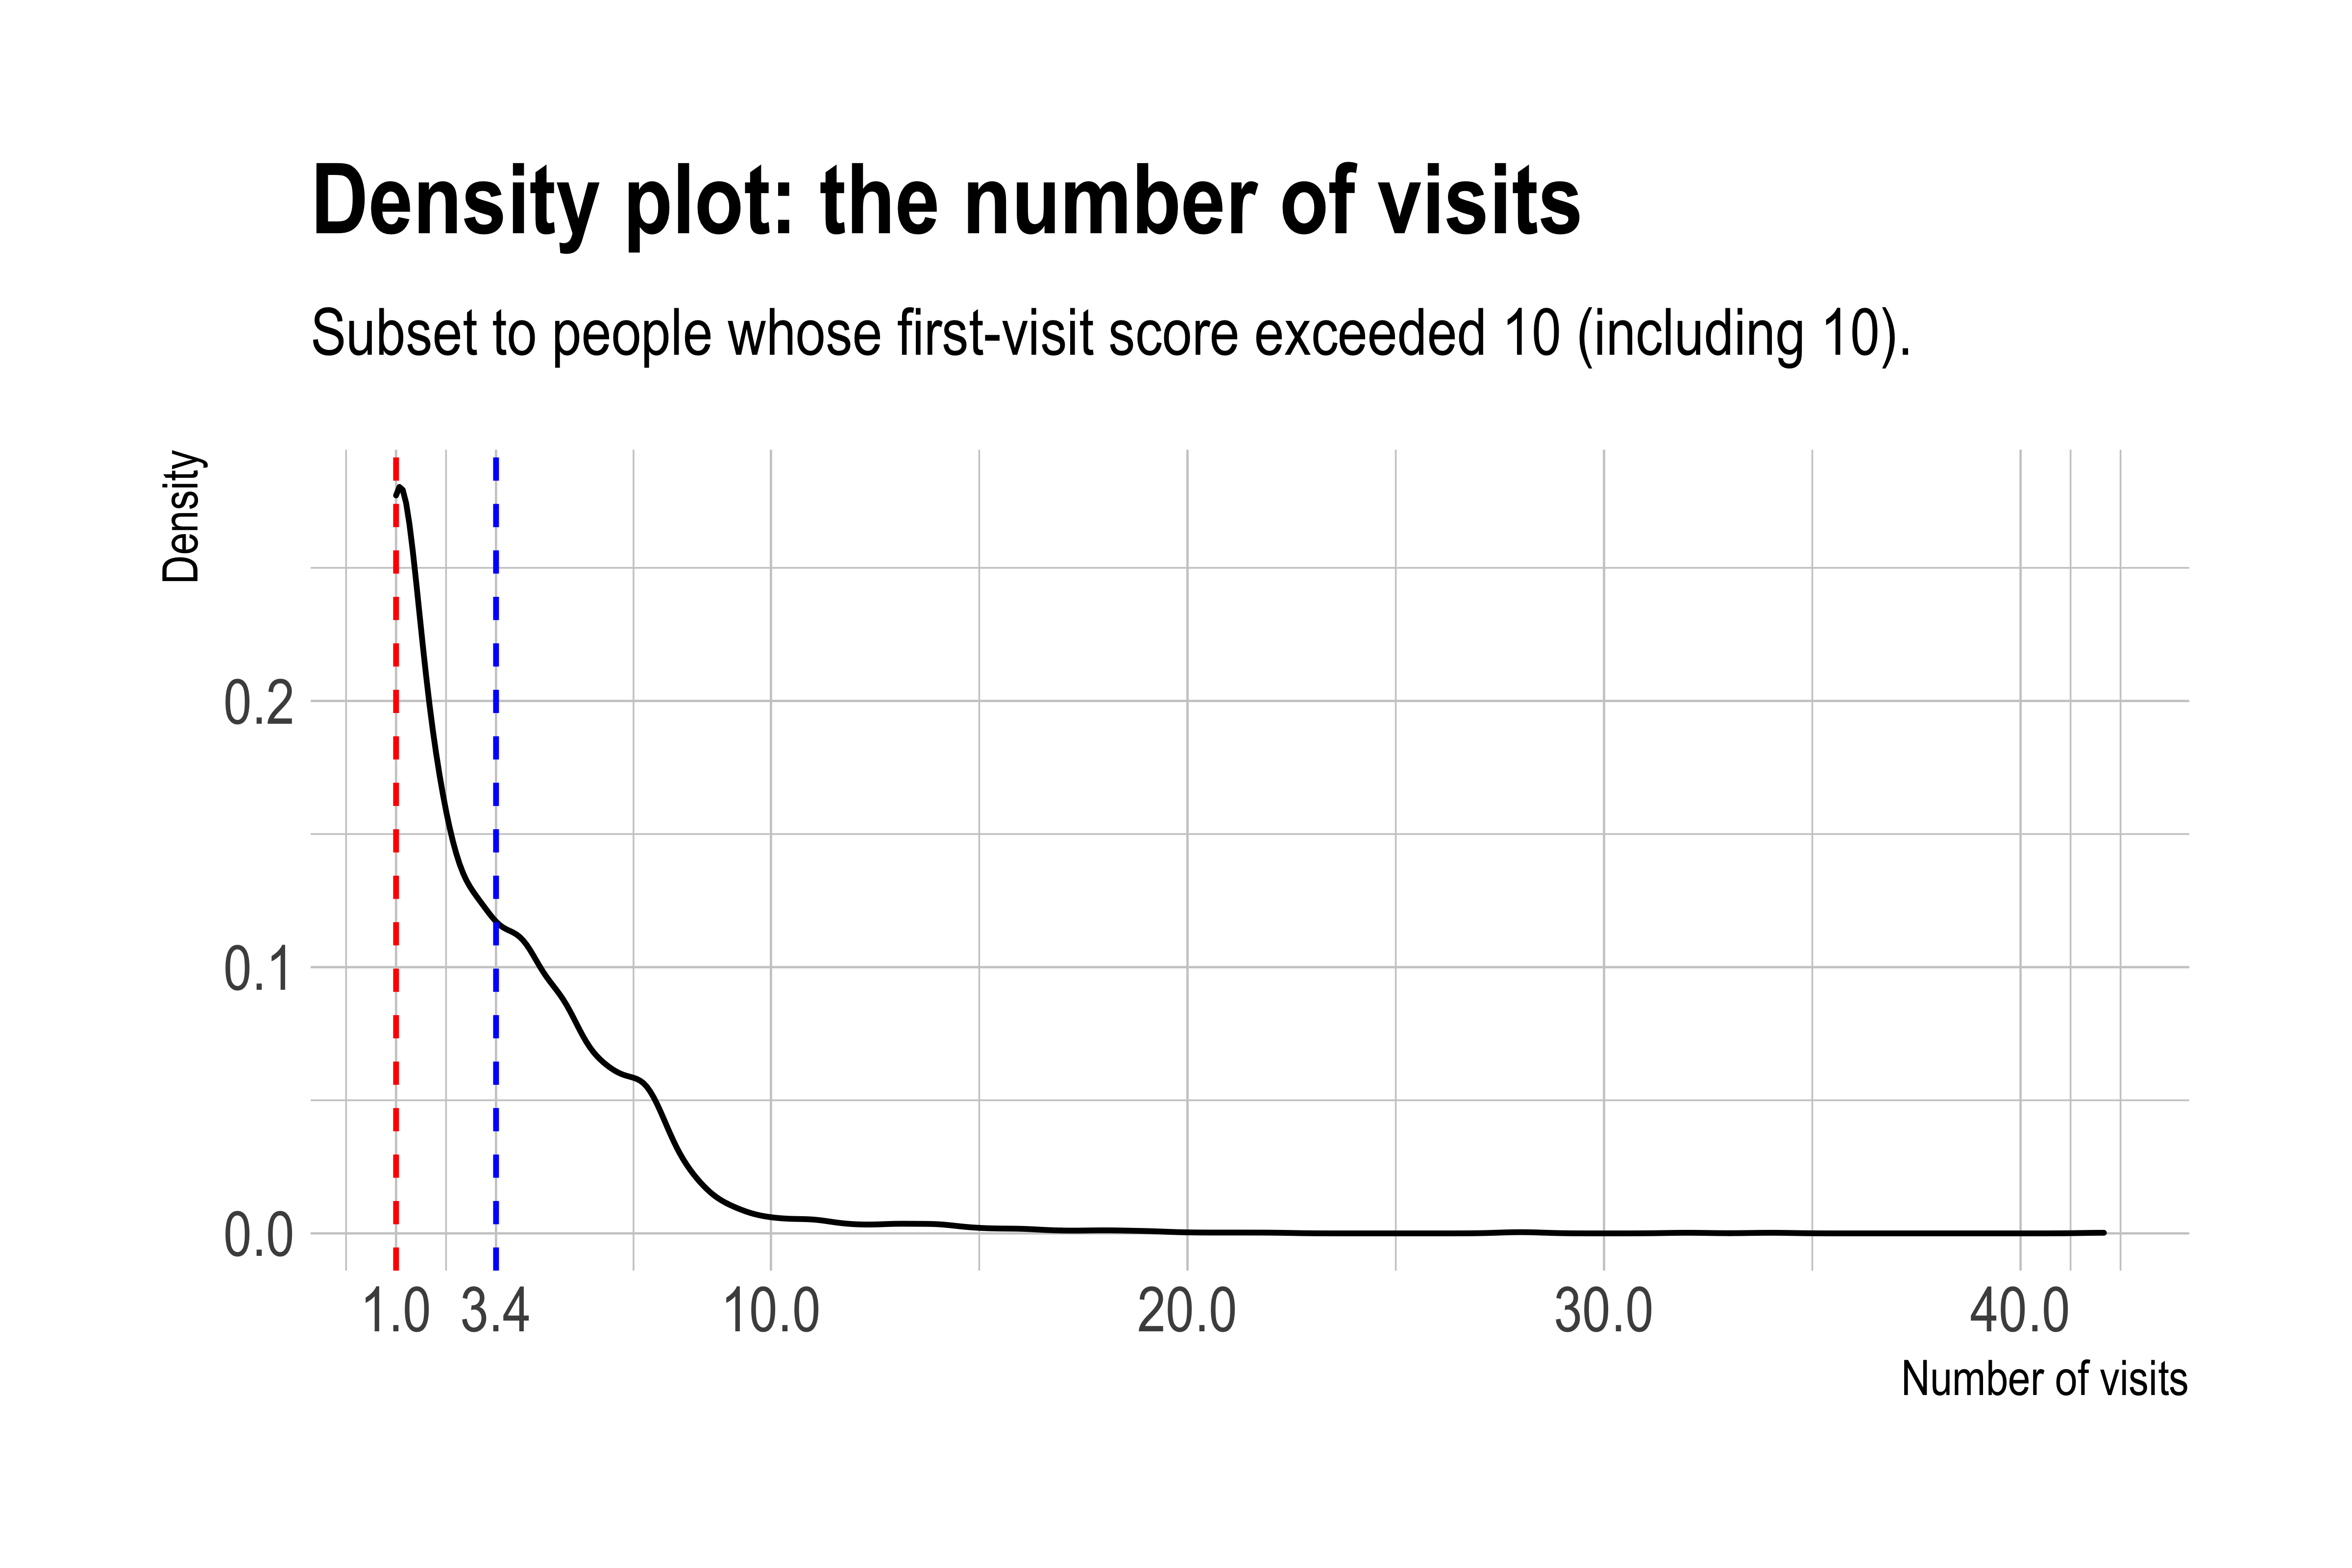
\includegraphics[width=\linewidth]{Figures/p7.png}
 		\caption{}\label{fig:p7}
 	\end{subfigure}
 	\hfill
 	\begin{subfigure}[h]{0.48\linewidth}
 		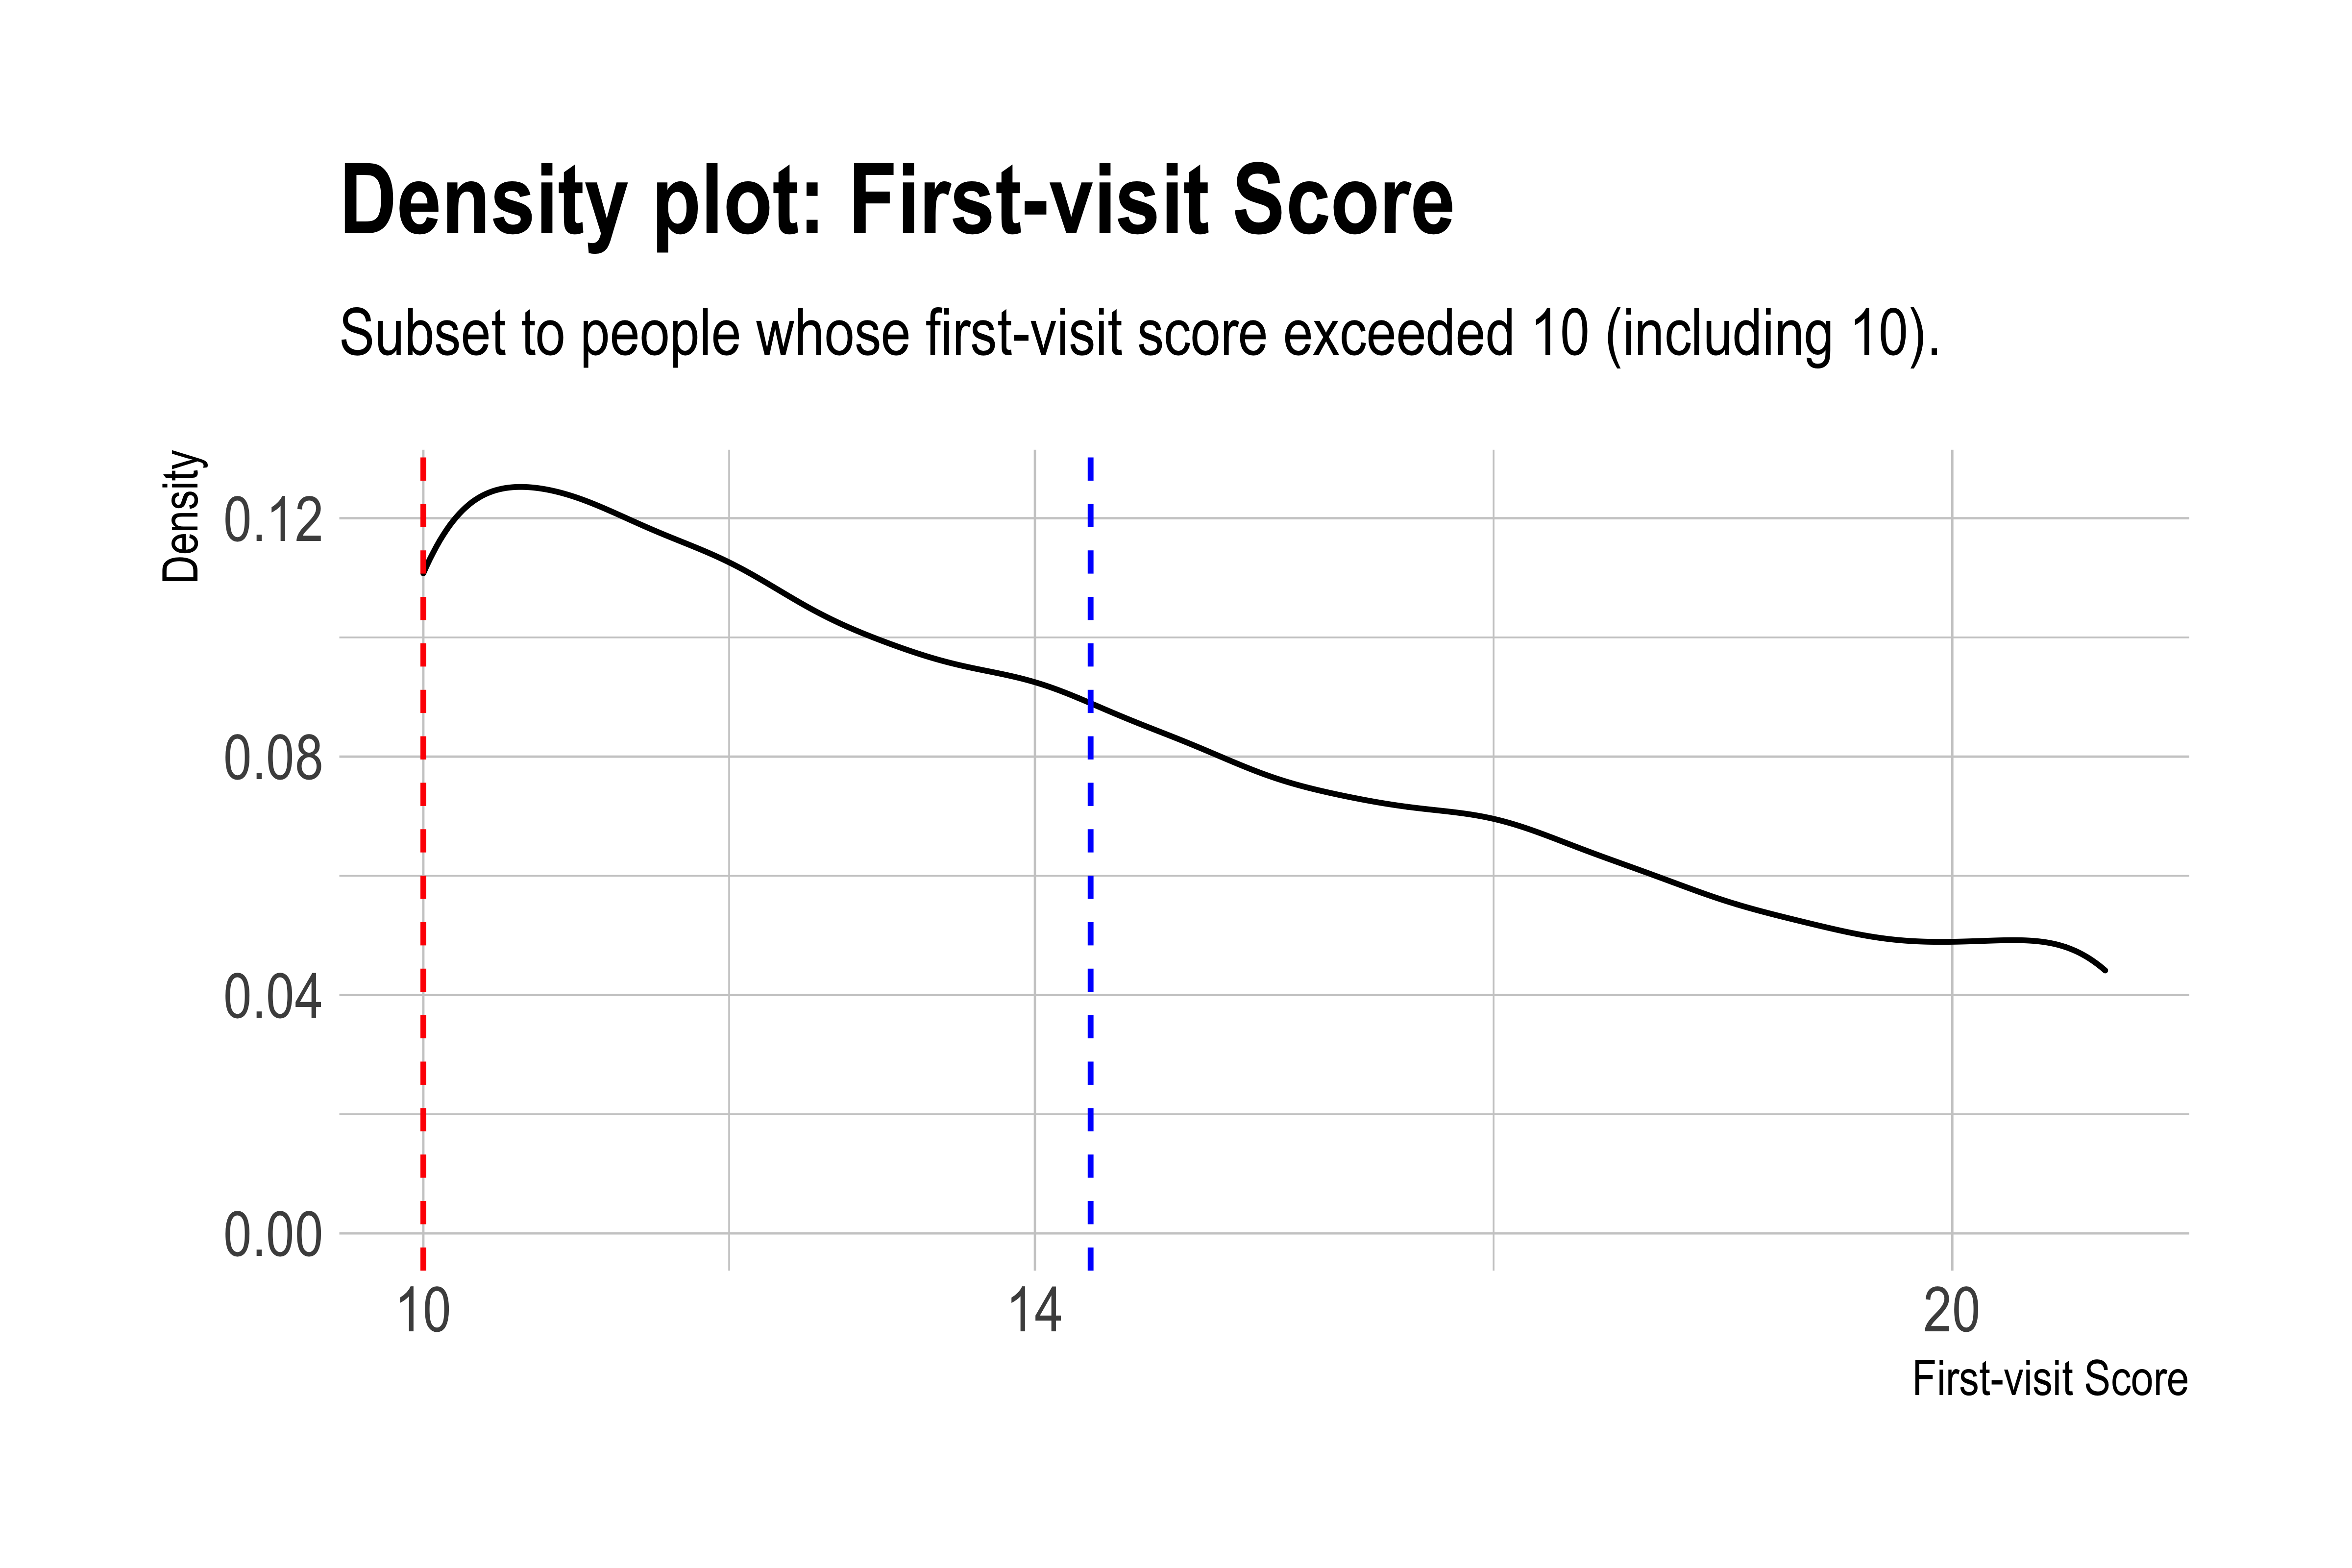
\includegraphics[width=\linewidth]{Figures/p9.png}
 		\caption{}\label{fig:p9}
 	\end{subfigure}
 	\hfill
 	\begin{subfigure}[h]{0.48\linewidth}
 		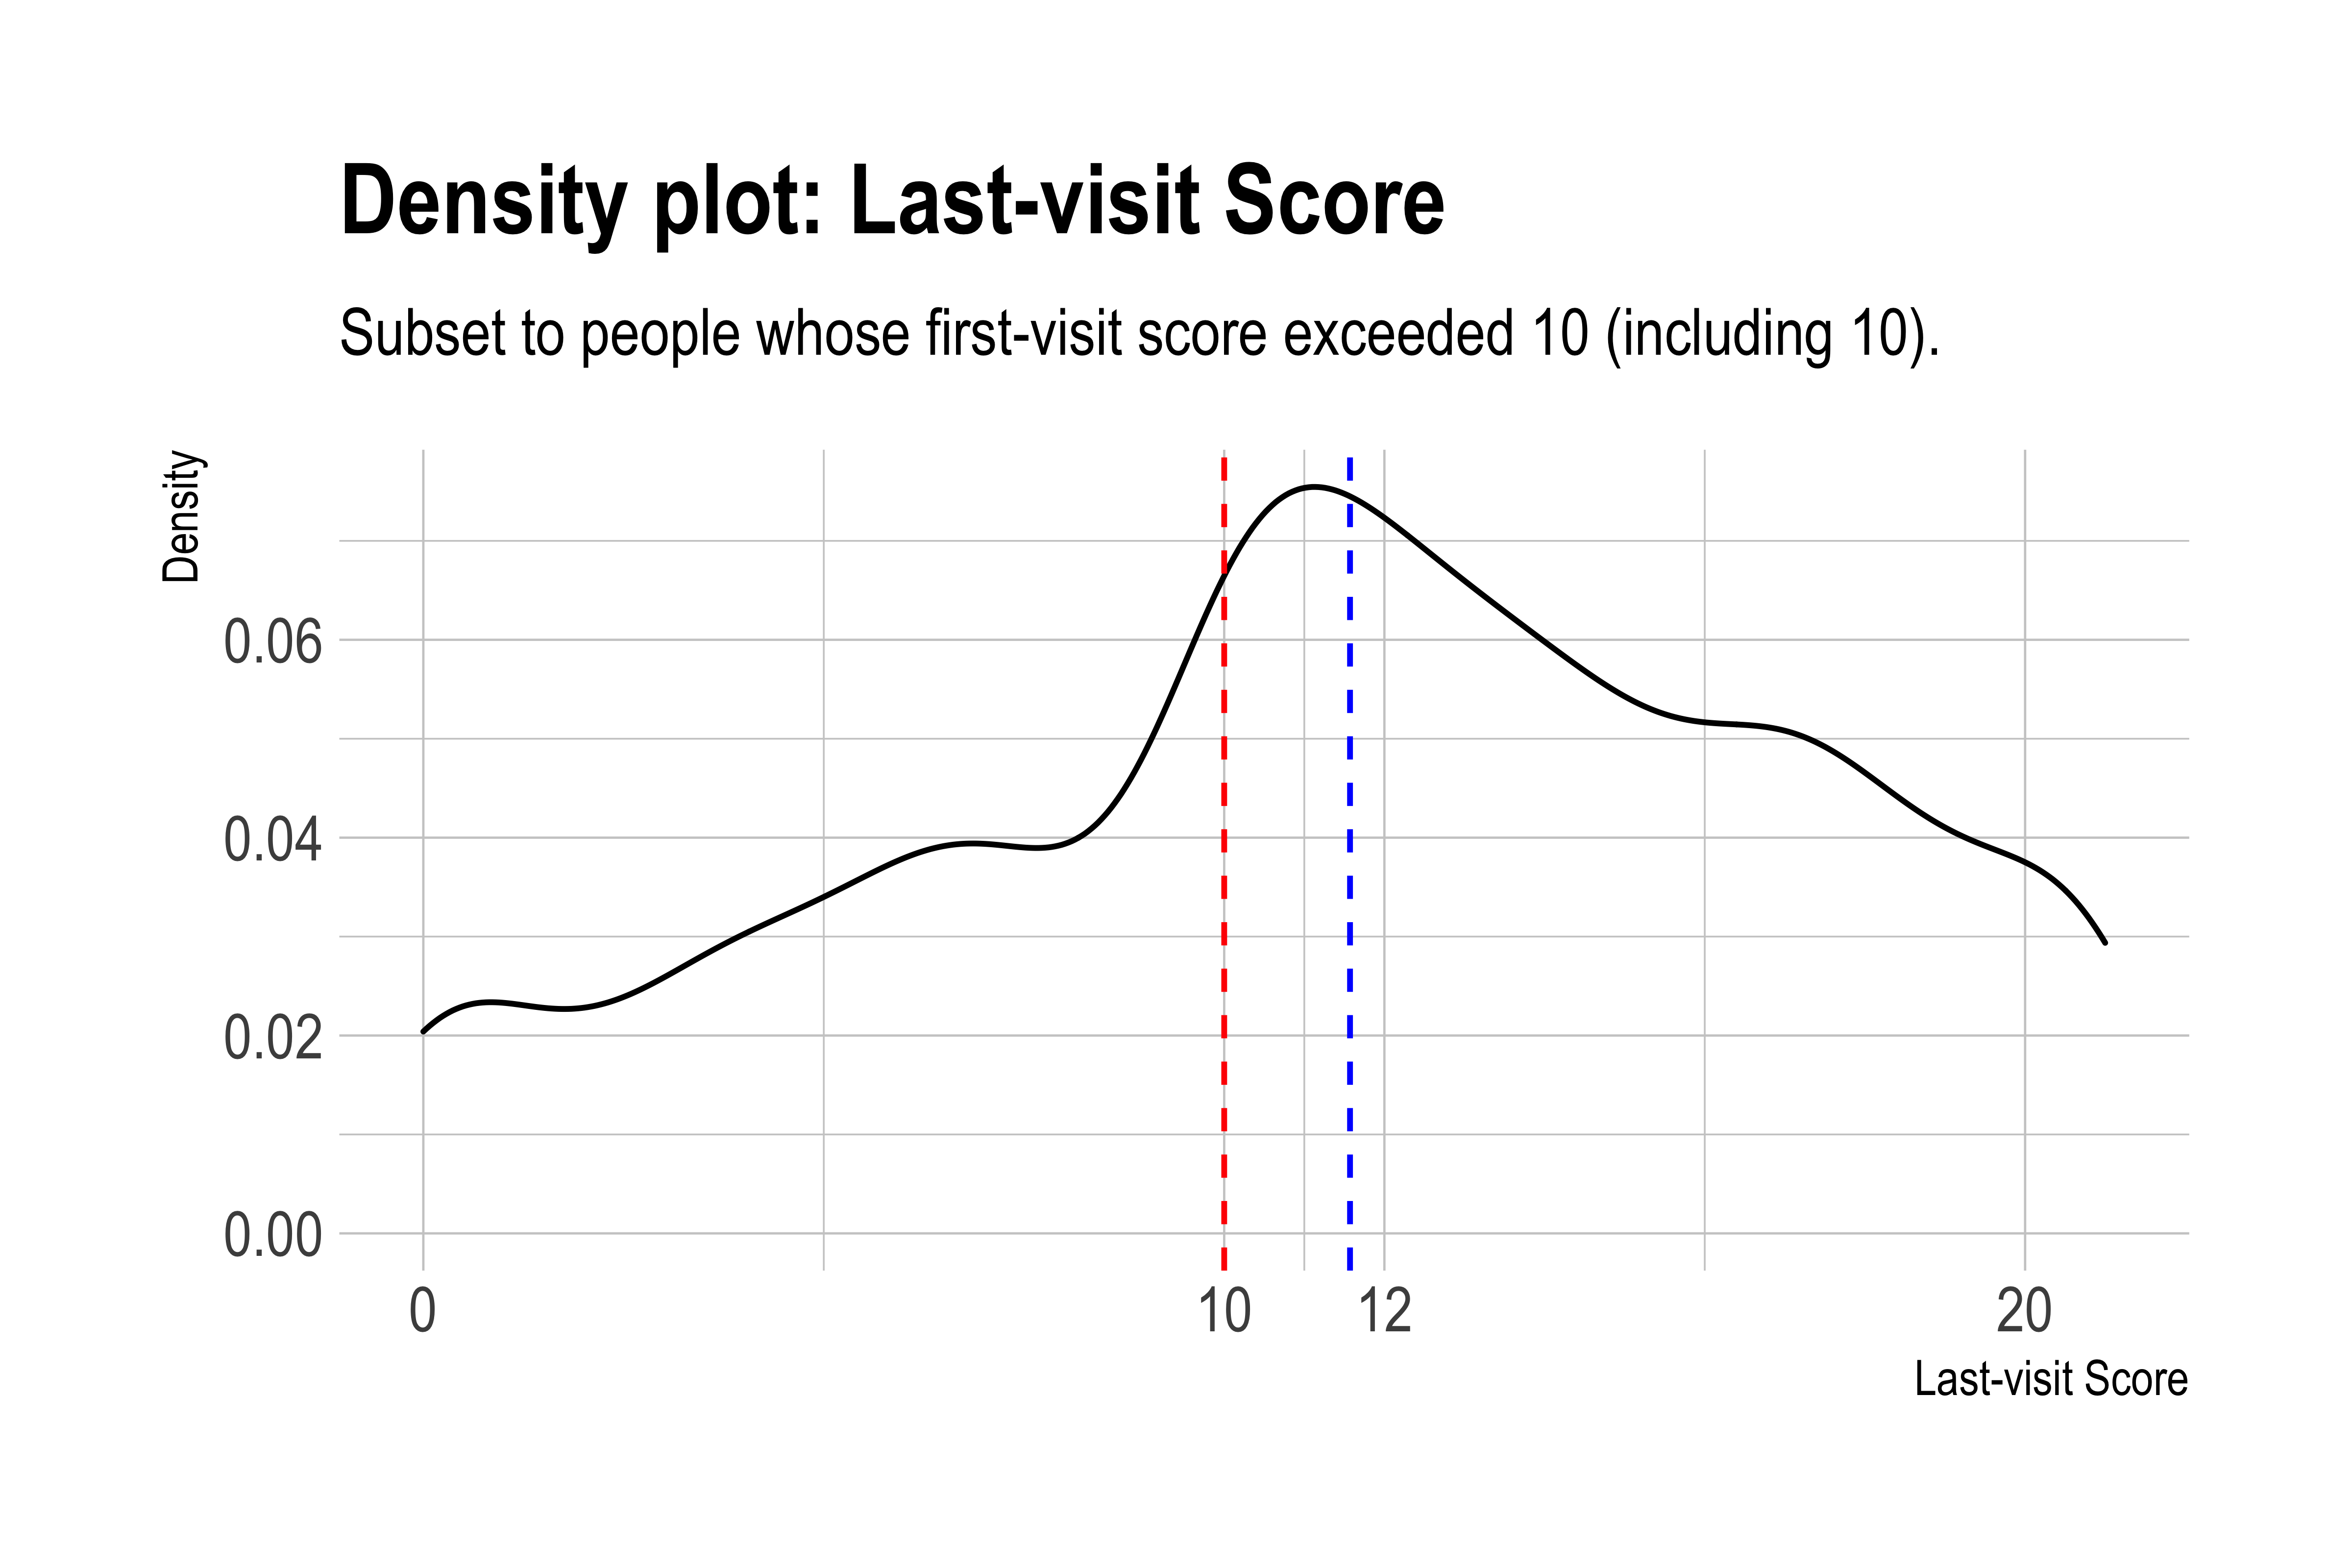
\includegraphics[width=\linewidth]{Figures/p10.png}
 		\caption{}\label{fig:p10}
 	\end{subfigure}
 	\hfill
 	\begin{subfigure}[h]{0.48\linewidth}
 		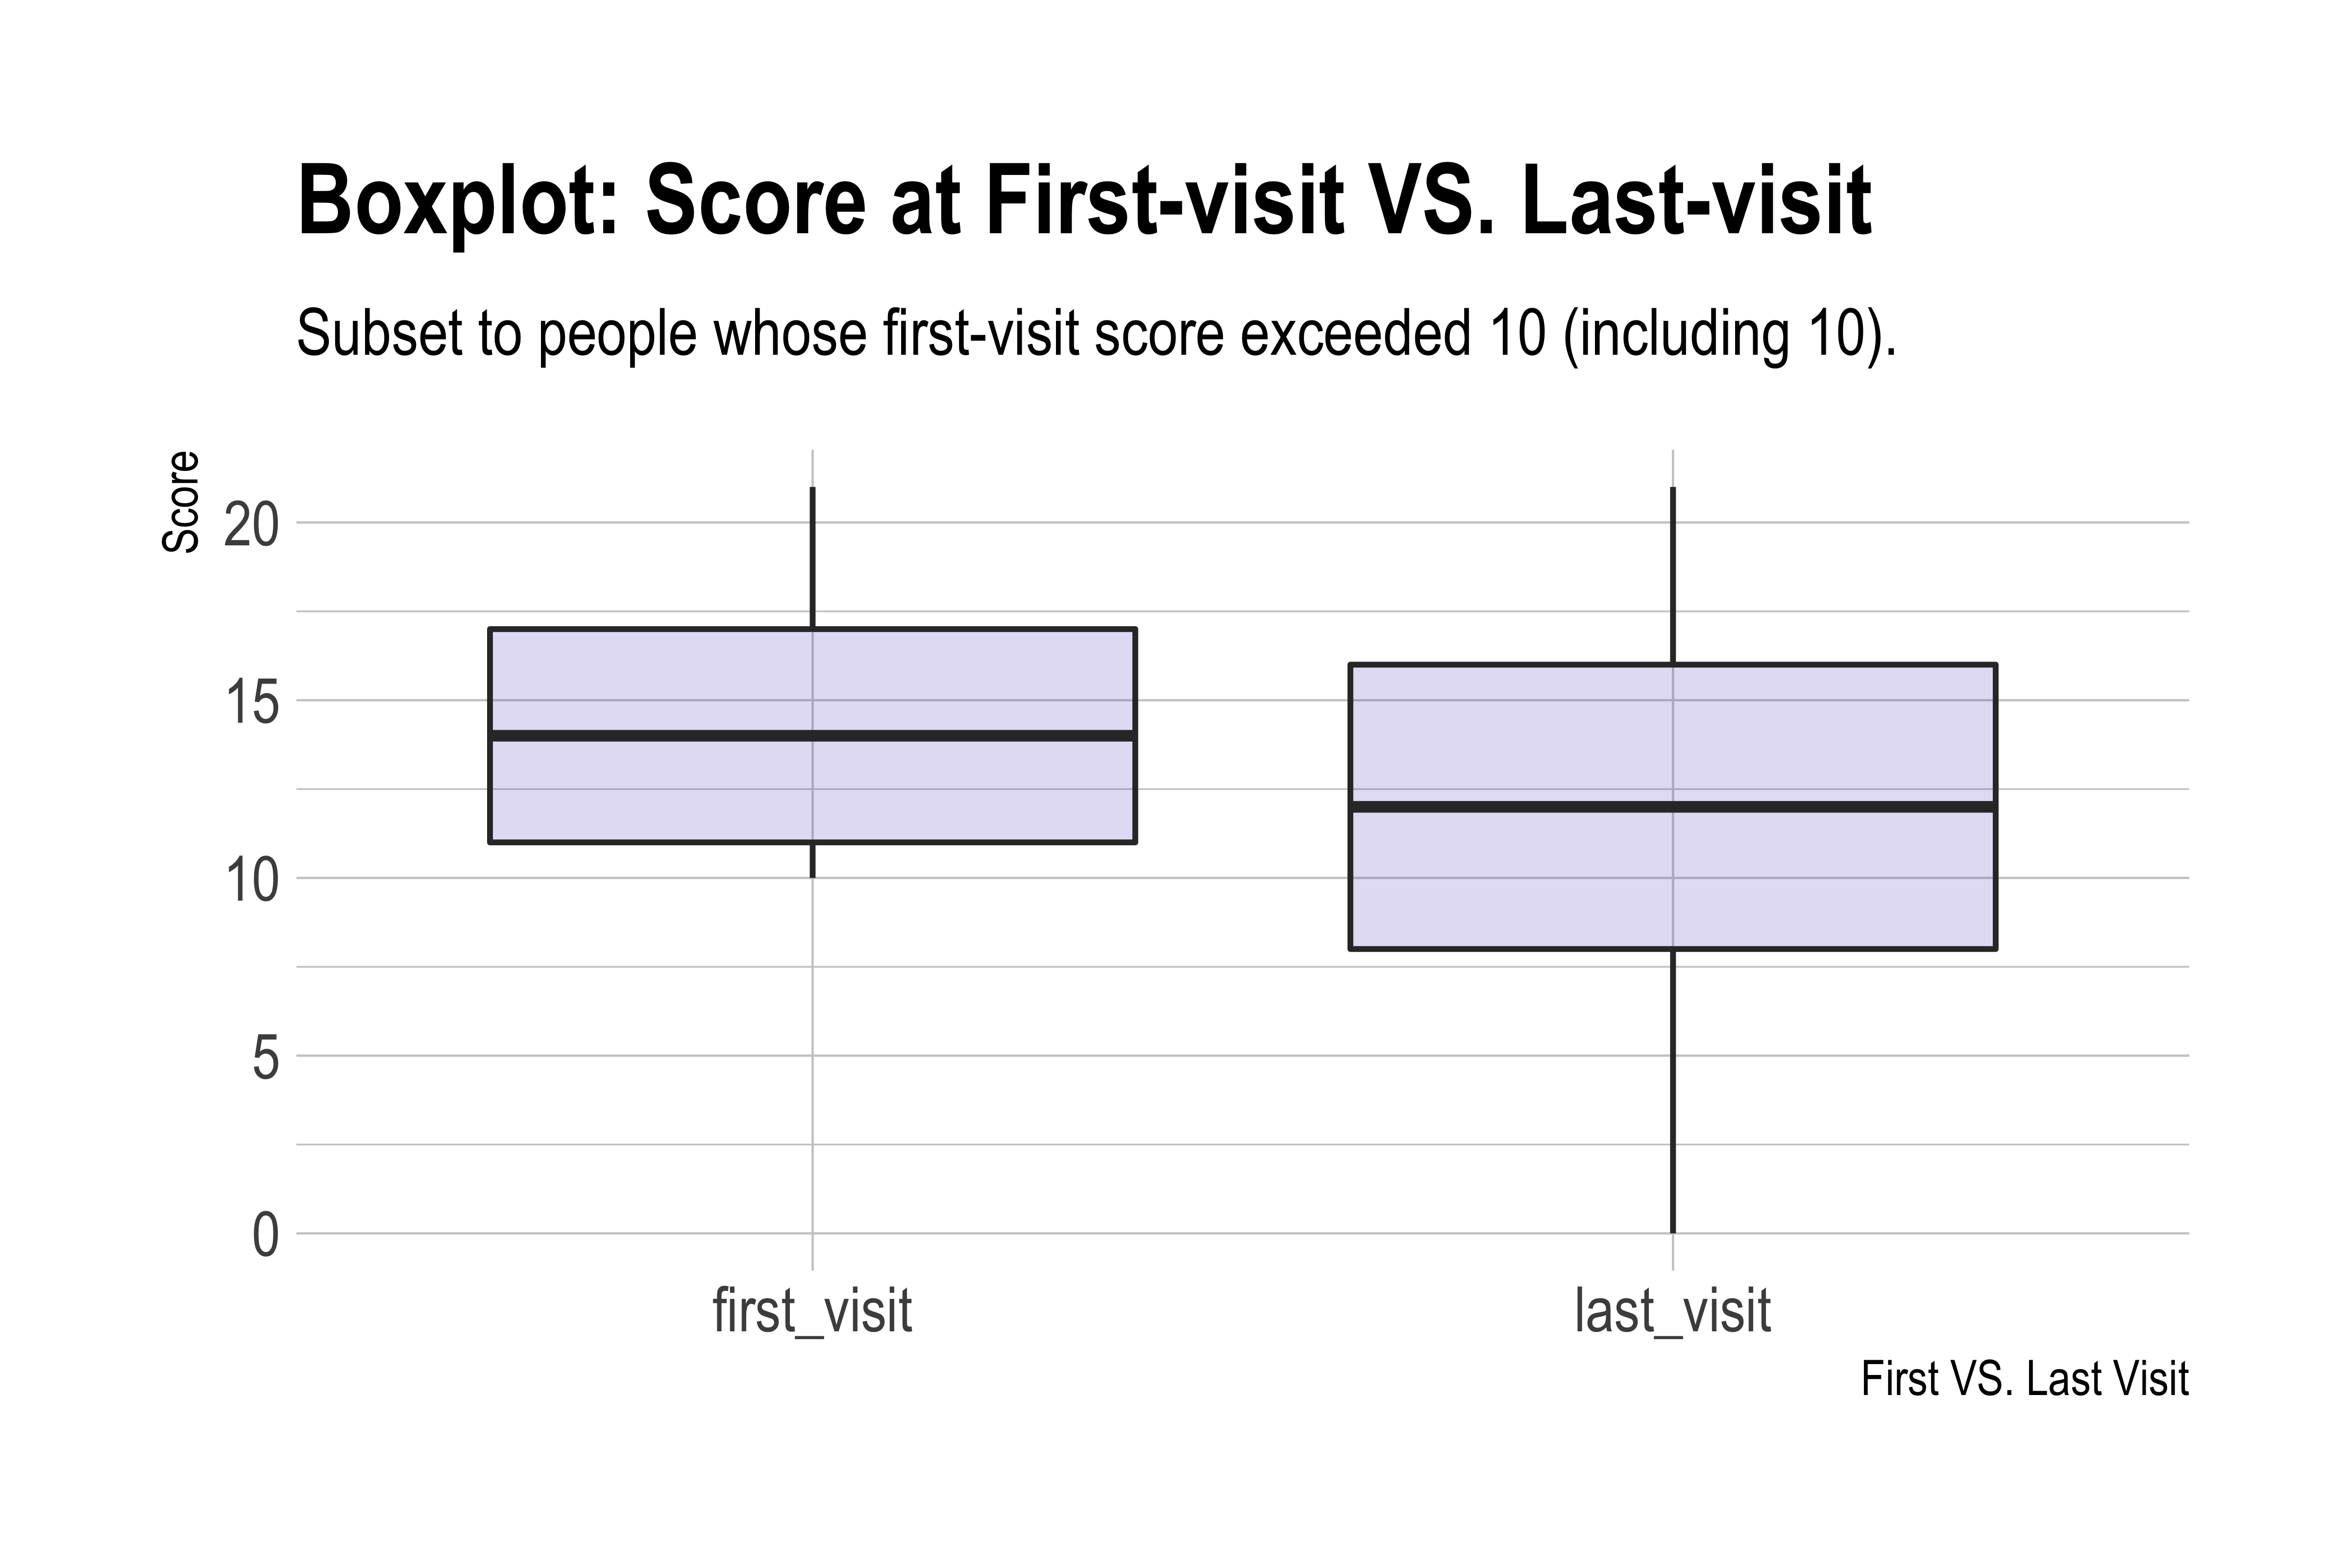
\includegraphics[width=\linewidth]{Figures/p6.png}
 		\caption{}\label{fig:p6}
 	\end{subfigure}
 \end{figure}

\section{Exploratory analysis} \label{ss:sec2}

Built on a better understanding of the dataset from the above descriptive distributions, let's dive deeper into possible ways that we could exploit. I mainly tried three methods.

\begin{enumerate}
	\item \textbf{Boxplot}\\
	Firstly, we can see from figure \ref{fig:p5} that patients in the full dataset who paid more than 4 clinical visits in general released their anxiety level until the last visit more than the overall level. Further limiting to our targeting patient group (recall that this contains patients whose anxiety score on the first-visit is equal to or larger than 10), we can see some interesting pattern in figure \ref{fig:p7}. In this boxplot, we compare the anxiety score on the last-visit between patients who are considered to have received "sufficient treatment" versus those who did not. Assuming that the nubmer of visits roughly demonstrate the magnitude of treatment, I set the standard of "sufficient" to be 3.4 visits (average visit frequency), 5 visits (third-quantile visit frequency), and 10 visits. For example, the middle boxplot in figure \ref{fig:p7} presents the anxiety score on the last-visit for patients who visited less than 5 times and patients who visited more than 5 times (including five times). Patients who are treated more (paid more clinical visits) substantially decreased their anxiety score at the last visit compared to those who visited the clinic fewer times. And visiting over 10 times seems to have a larger effect.
	
	 \begin{figure}[htb!]
		\caption{Box plots}\label{fig:picture3}
		\begin{subfigure}[h]{0.48\linewidth}
			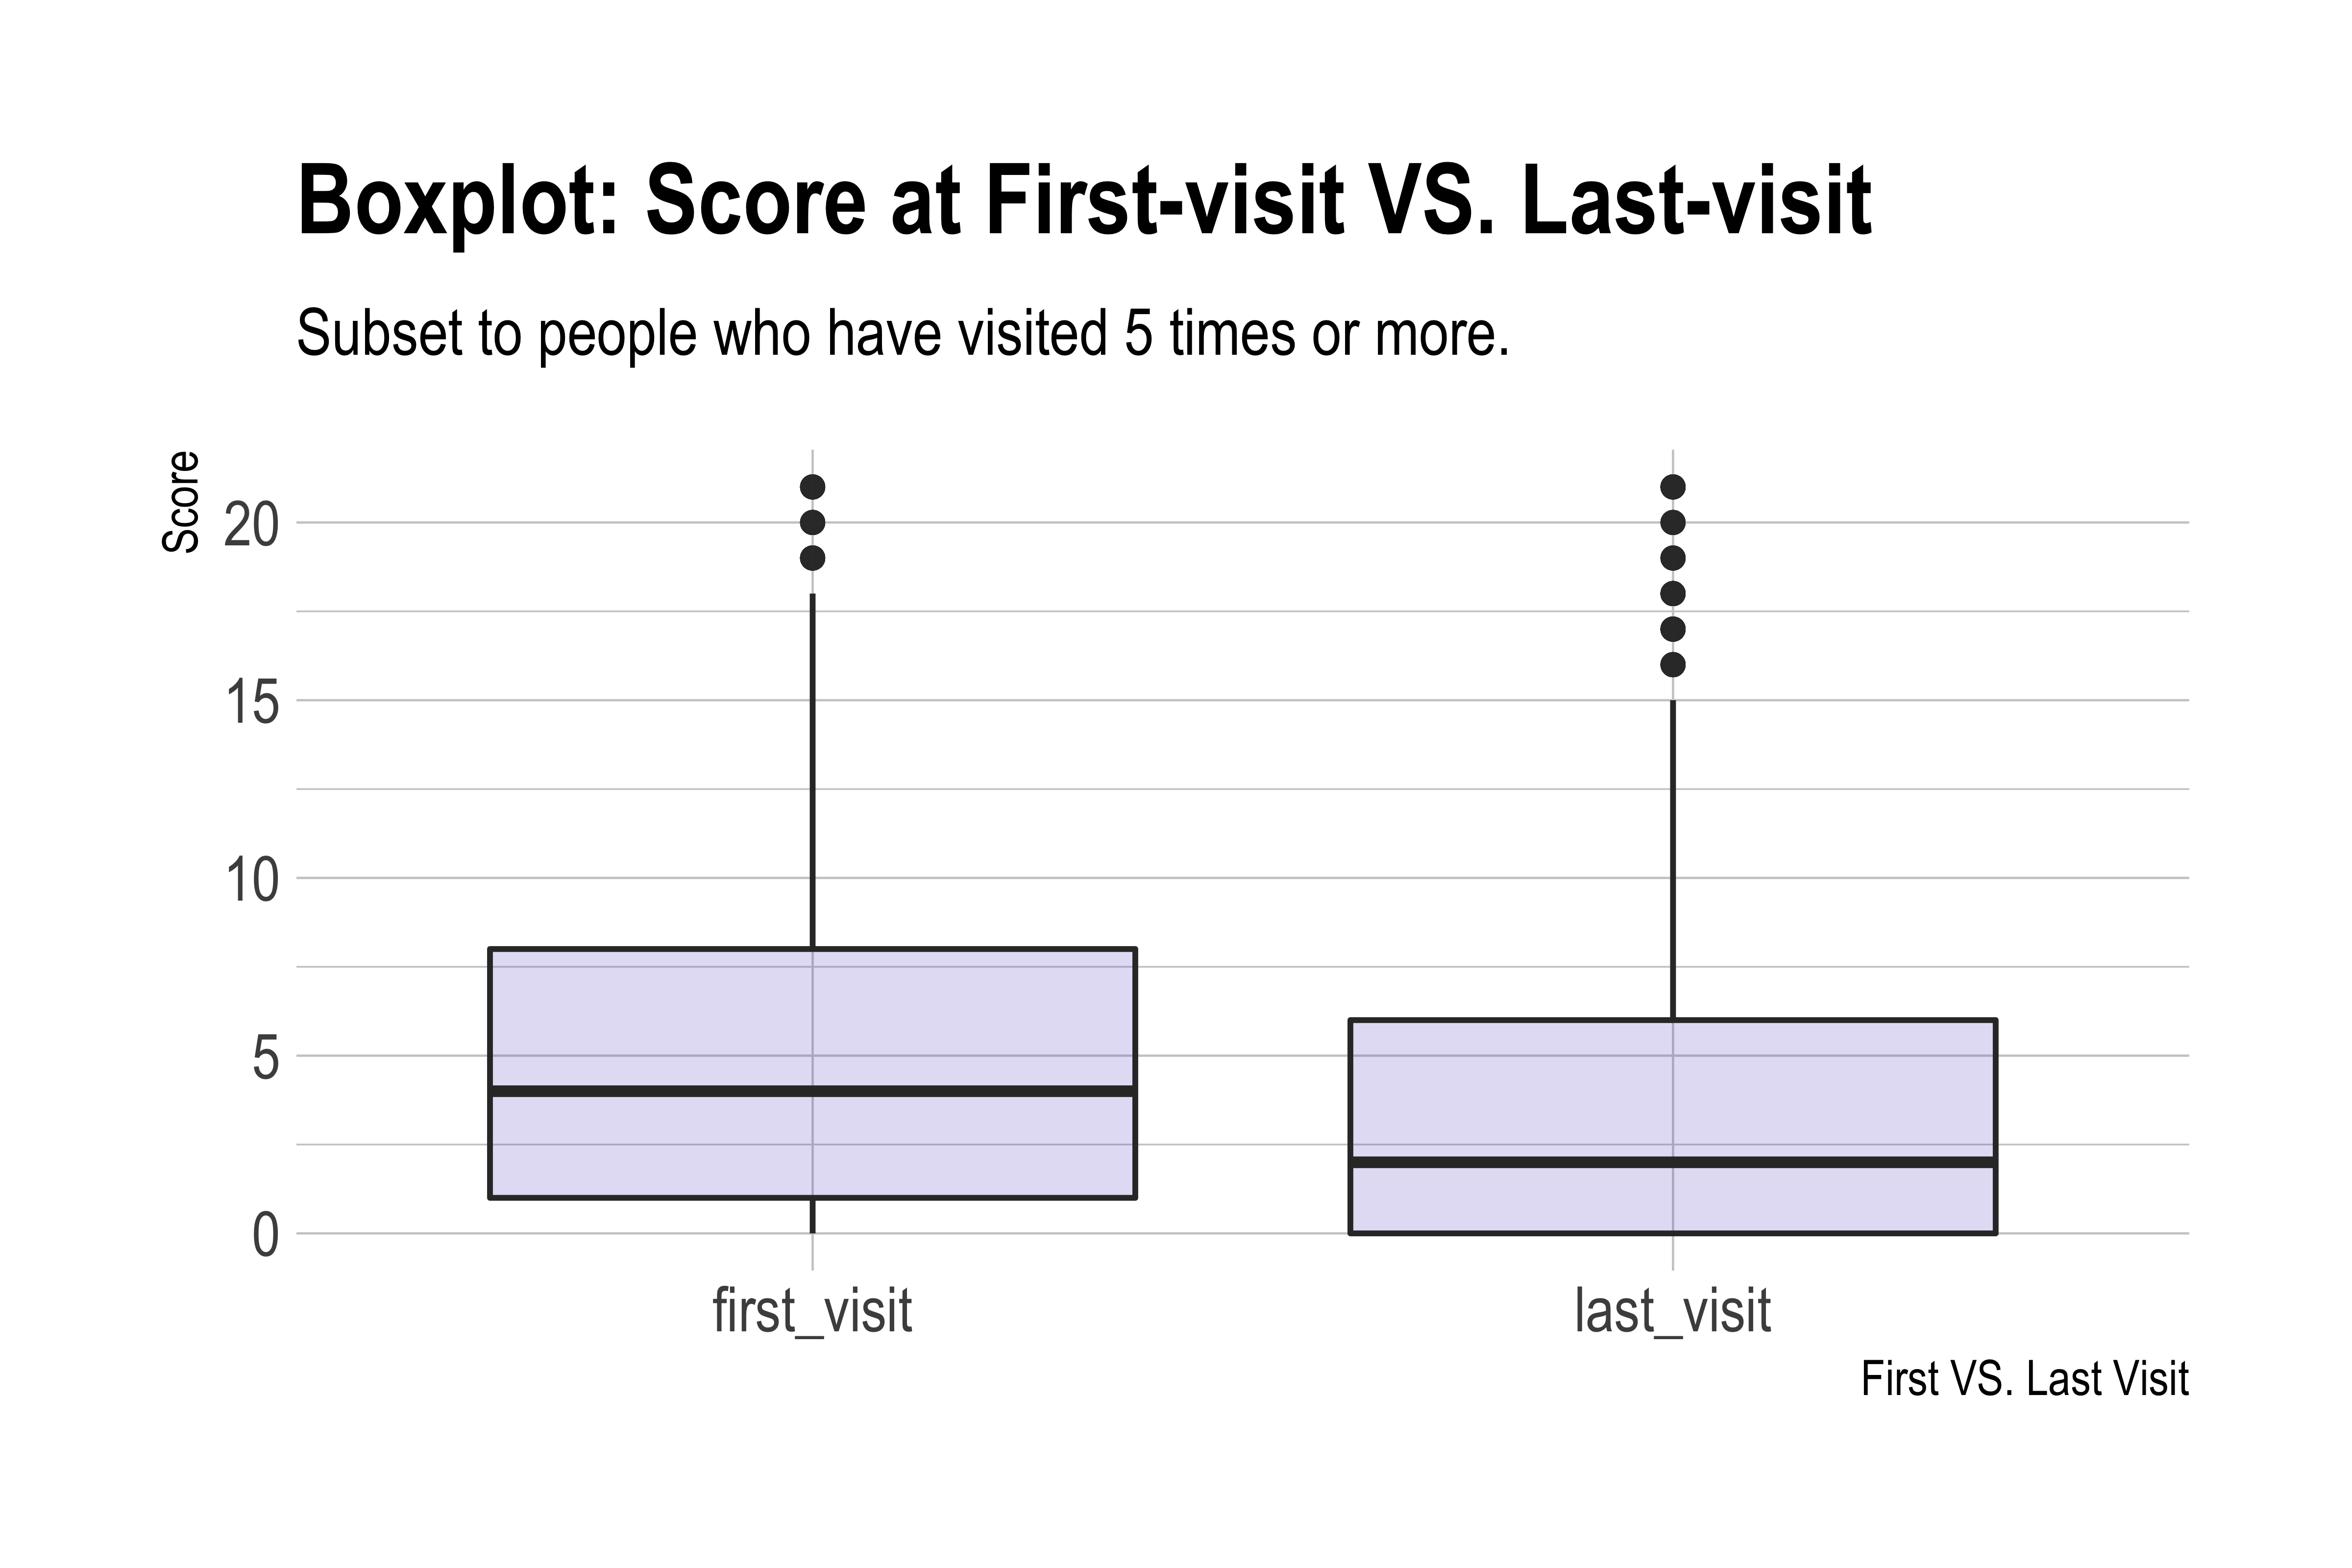
\includegraphics[width=\linewidth]{Figures/p5.png}
			\caption{}\label{fig:p5}
		\end{subfigure}
		\hfill
		\begin{subfigure}[h]{0.48\linewidth}
			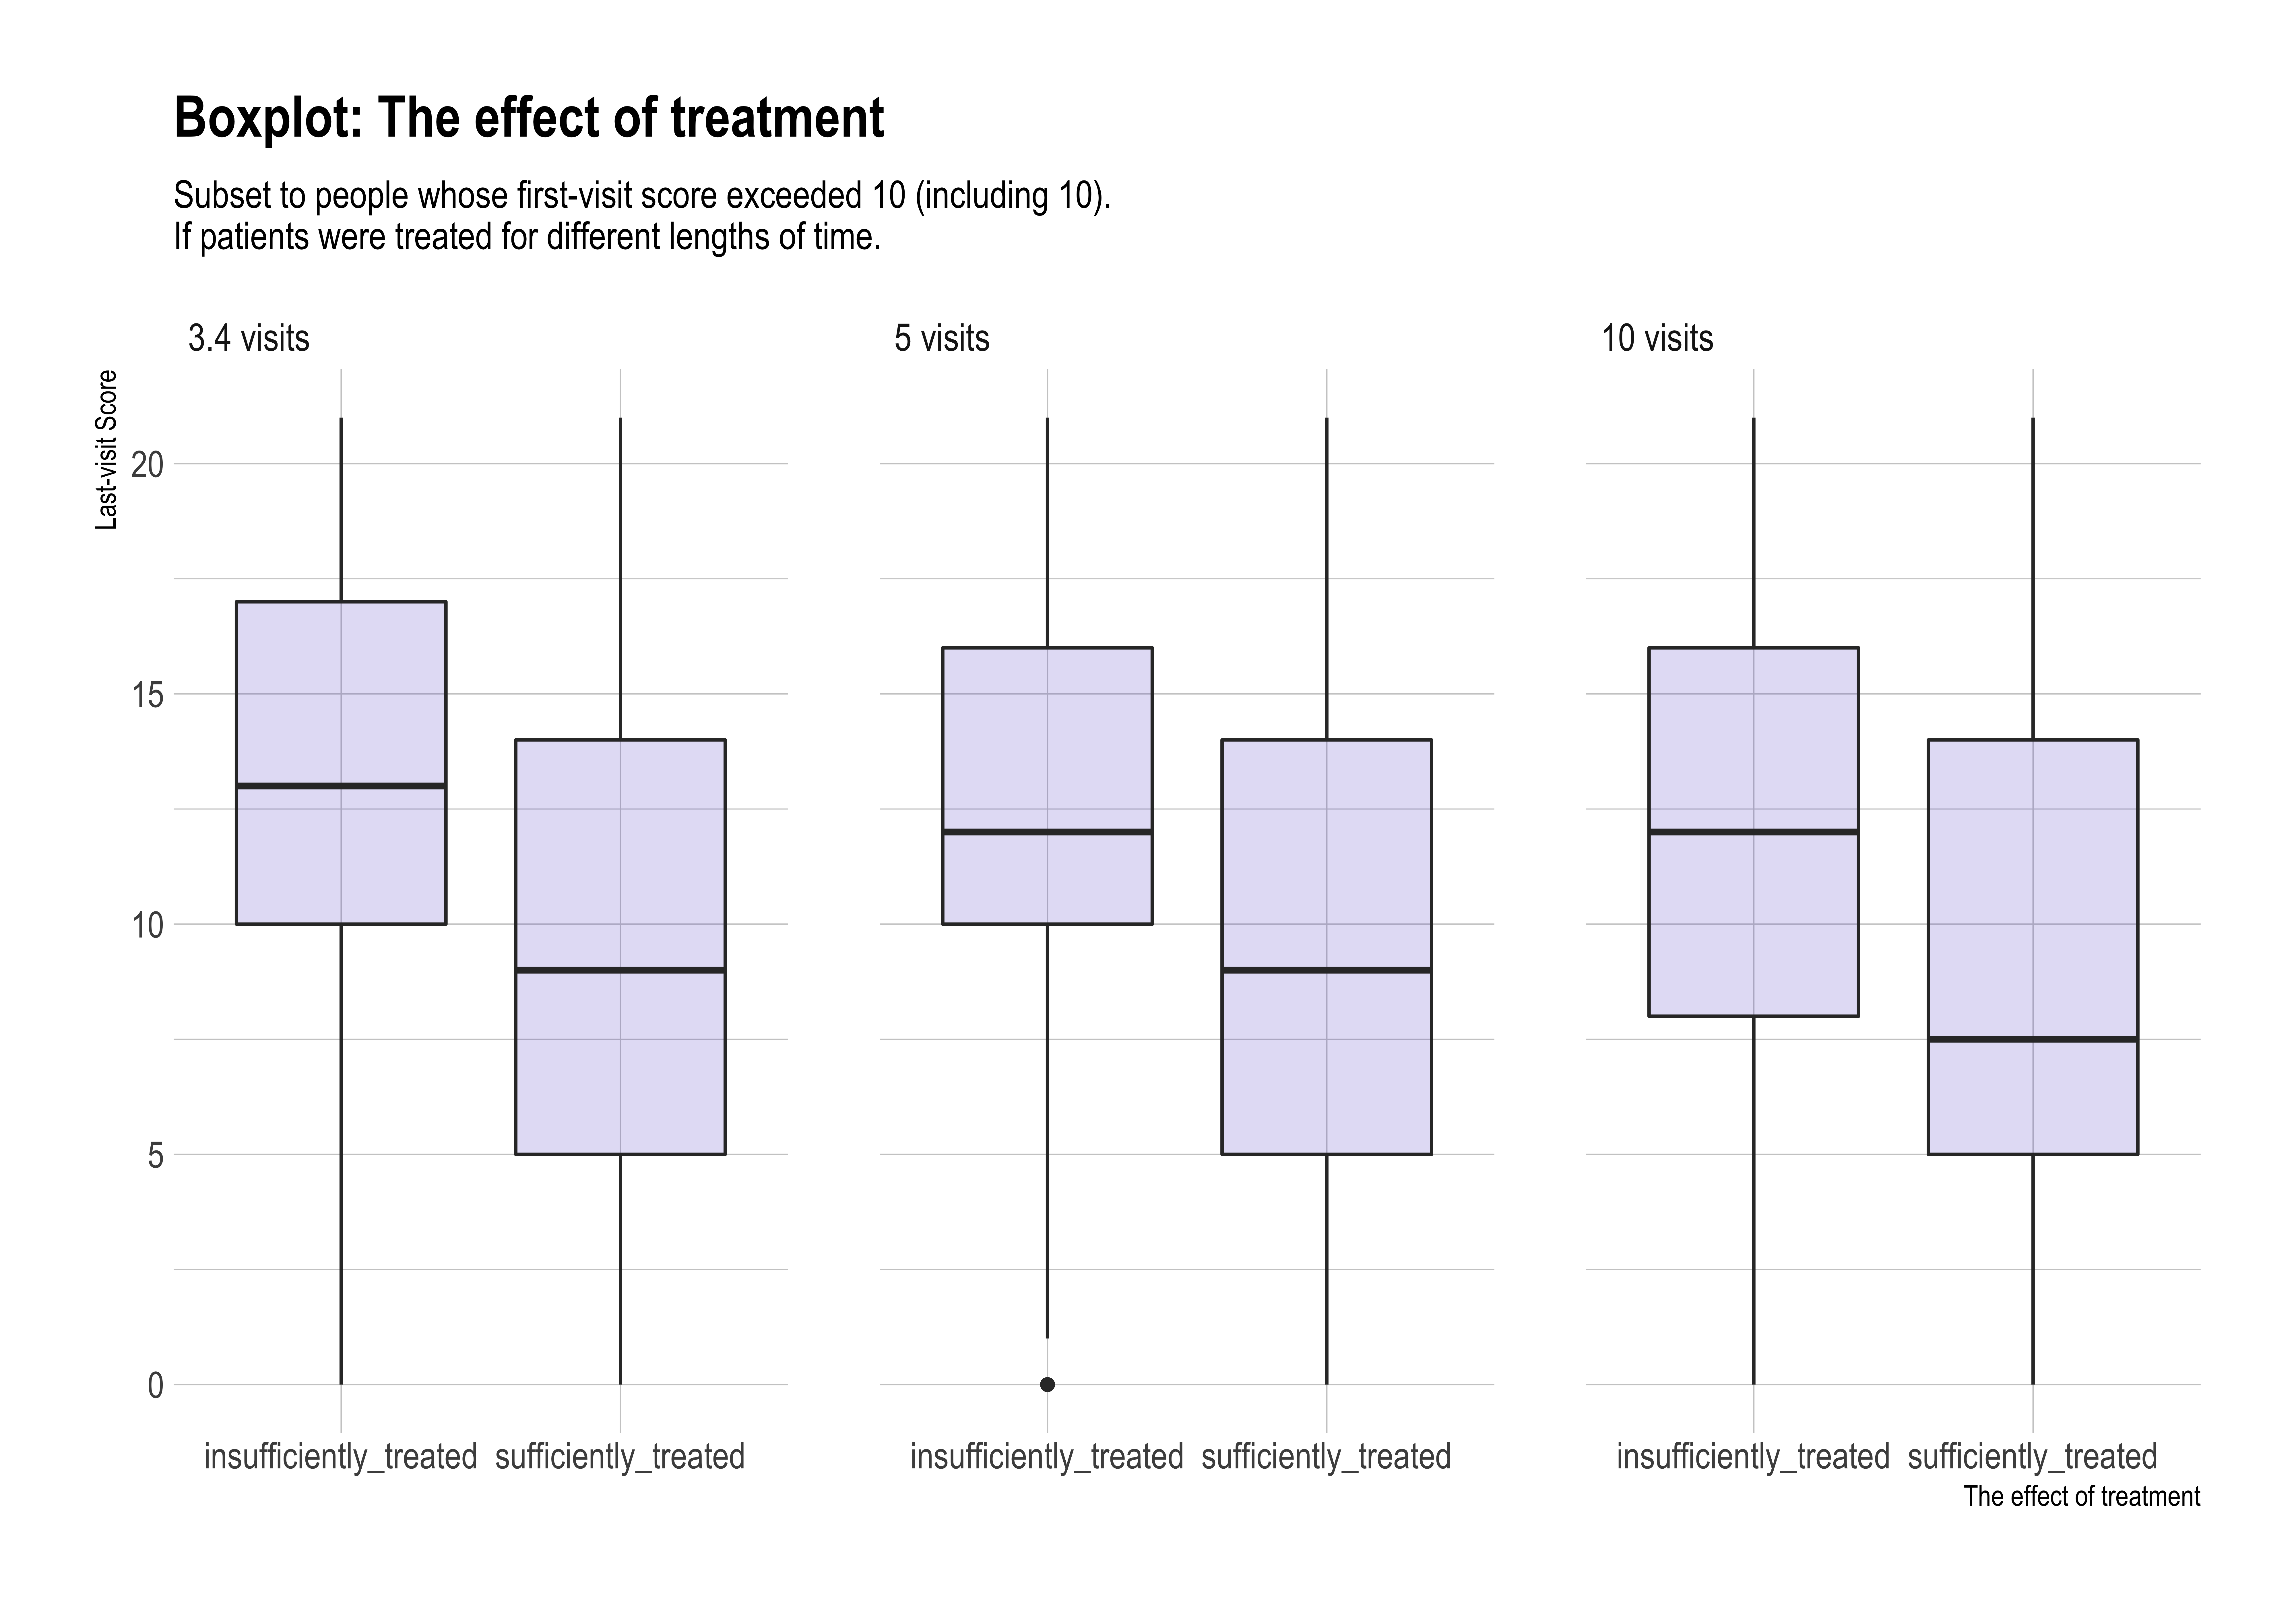
\includegraphics[width=\linewidth]{Figures/p8.png}
			\caption{}\label{fig:p8}
		\end{subfigure}
	\end{figure}

	\item \textbf{Linear regression}\\
	
	Take each visits into consideration instead of restricting to the comparison of first and last visit. I harmonized the specific visiting date into numbered visit time. With that said, x-axis represents the first visit, the second visit, the third visit, ..., all the way to the last visit. Y axis is the anxiety score on each visit. Each point in the plot represents a visit score for one patient. By running a simple linear regression, we obtains a statistically significant coefficient of -0.38. This means that each one more clinical visit could decrease the anxiety score by 0.38, although the adjusted $R^2$ is quite small. The negative correlation (R = -0.23) also suggests that more visits are associated with lower anxiety score. Note that both correlation and regression coefficients only reveal the internal association, causal effects could not be drawn.
	
	 \begin{figure}[htb!]
		\caption{Linear regression}\label{fig:picture4}
		\centering
		\begin{subfigure}[h]{0.48\linewidth}
			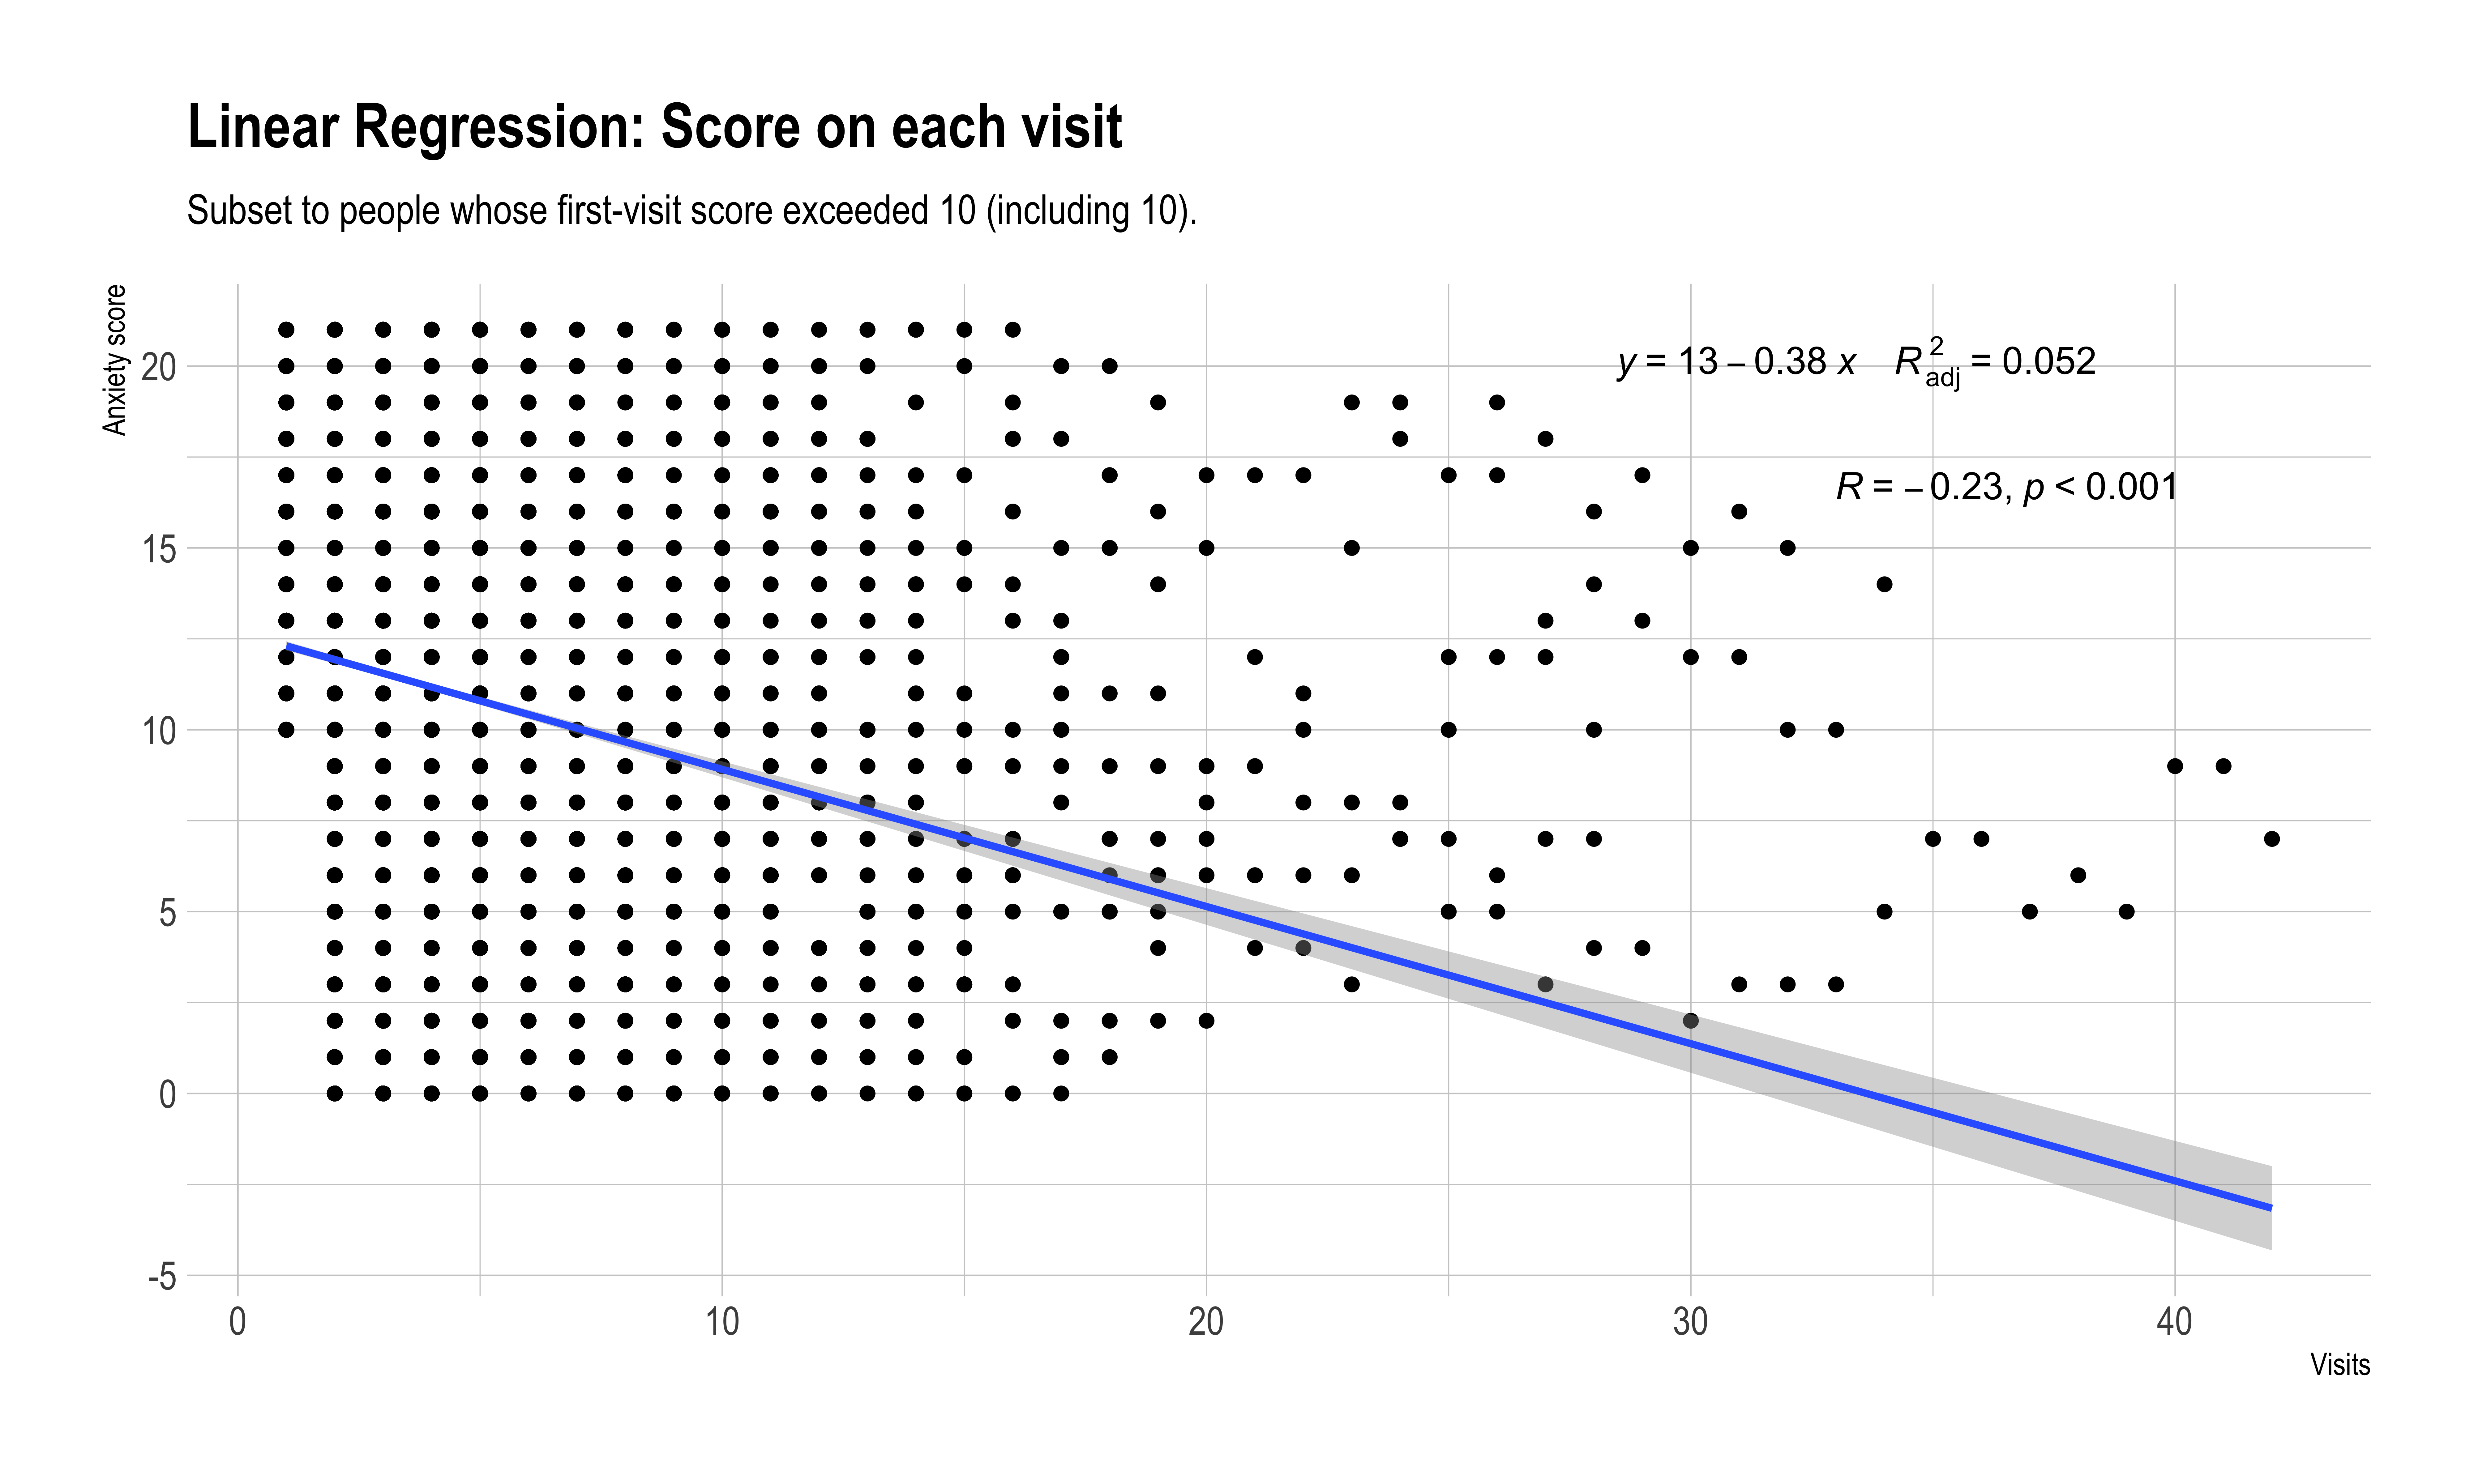
\includegraphics[width=\linewidth]{Figures/pp1.png}
			\caption{}\label{fig:pp1}
		\end{subfigure}
	\end{figure}

	\item \textbf{logistic regression}\\
	
	Using the dichtomous "improve" variable as the dependent variable, I further conducted logistic regression. The independent variable here is the number of visits. Logistic regression usually reveals the probability distribution of possible binary outcomes. Interestingly, we obtains a statistically significant coefficient of 0.52. This means that patients could be $e^{0.52}$ = 1.68 times more likely to have improvements, by which we mean a lower anxiety score at the last-visit compared to the first-visit.

	 \begin{figure}[htb!]
		\caption{Logistic regression}\label{fig:picture5}
		\centering
		\begin{subfigure}[h]{0.48\linewidth}
			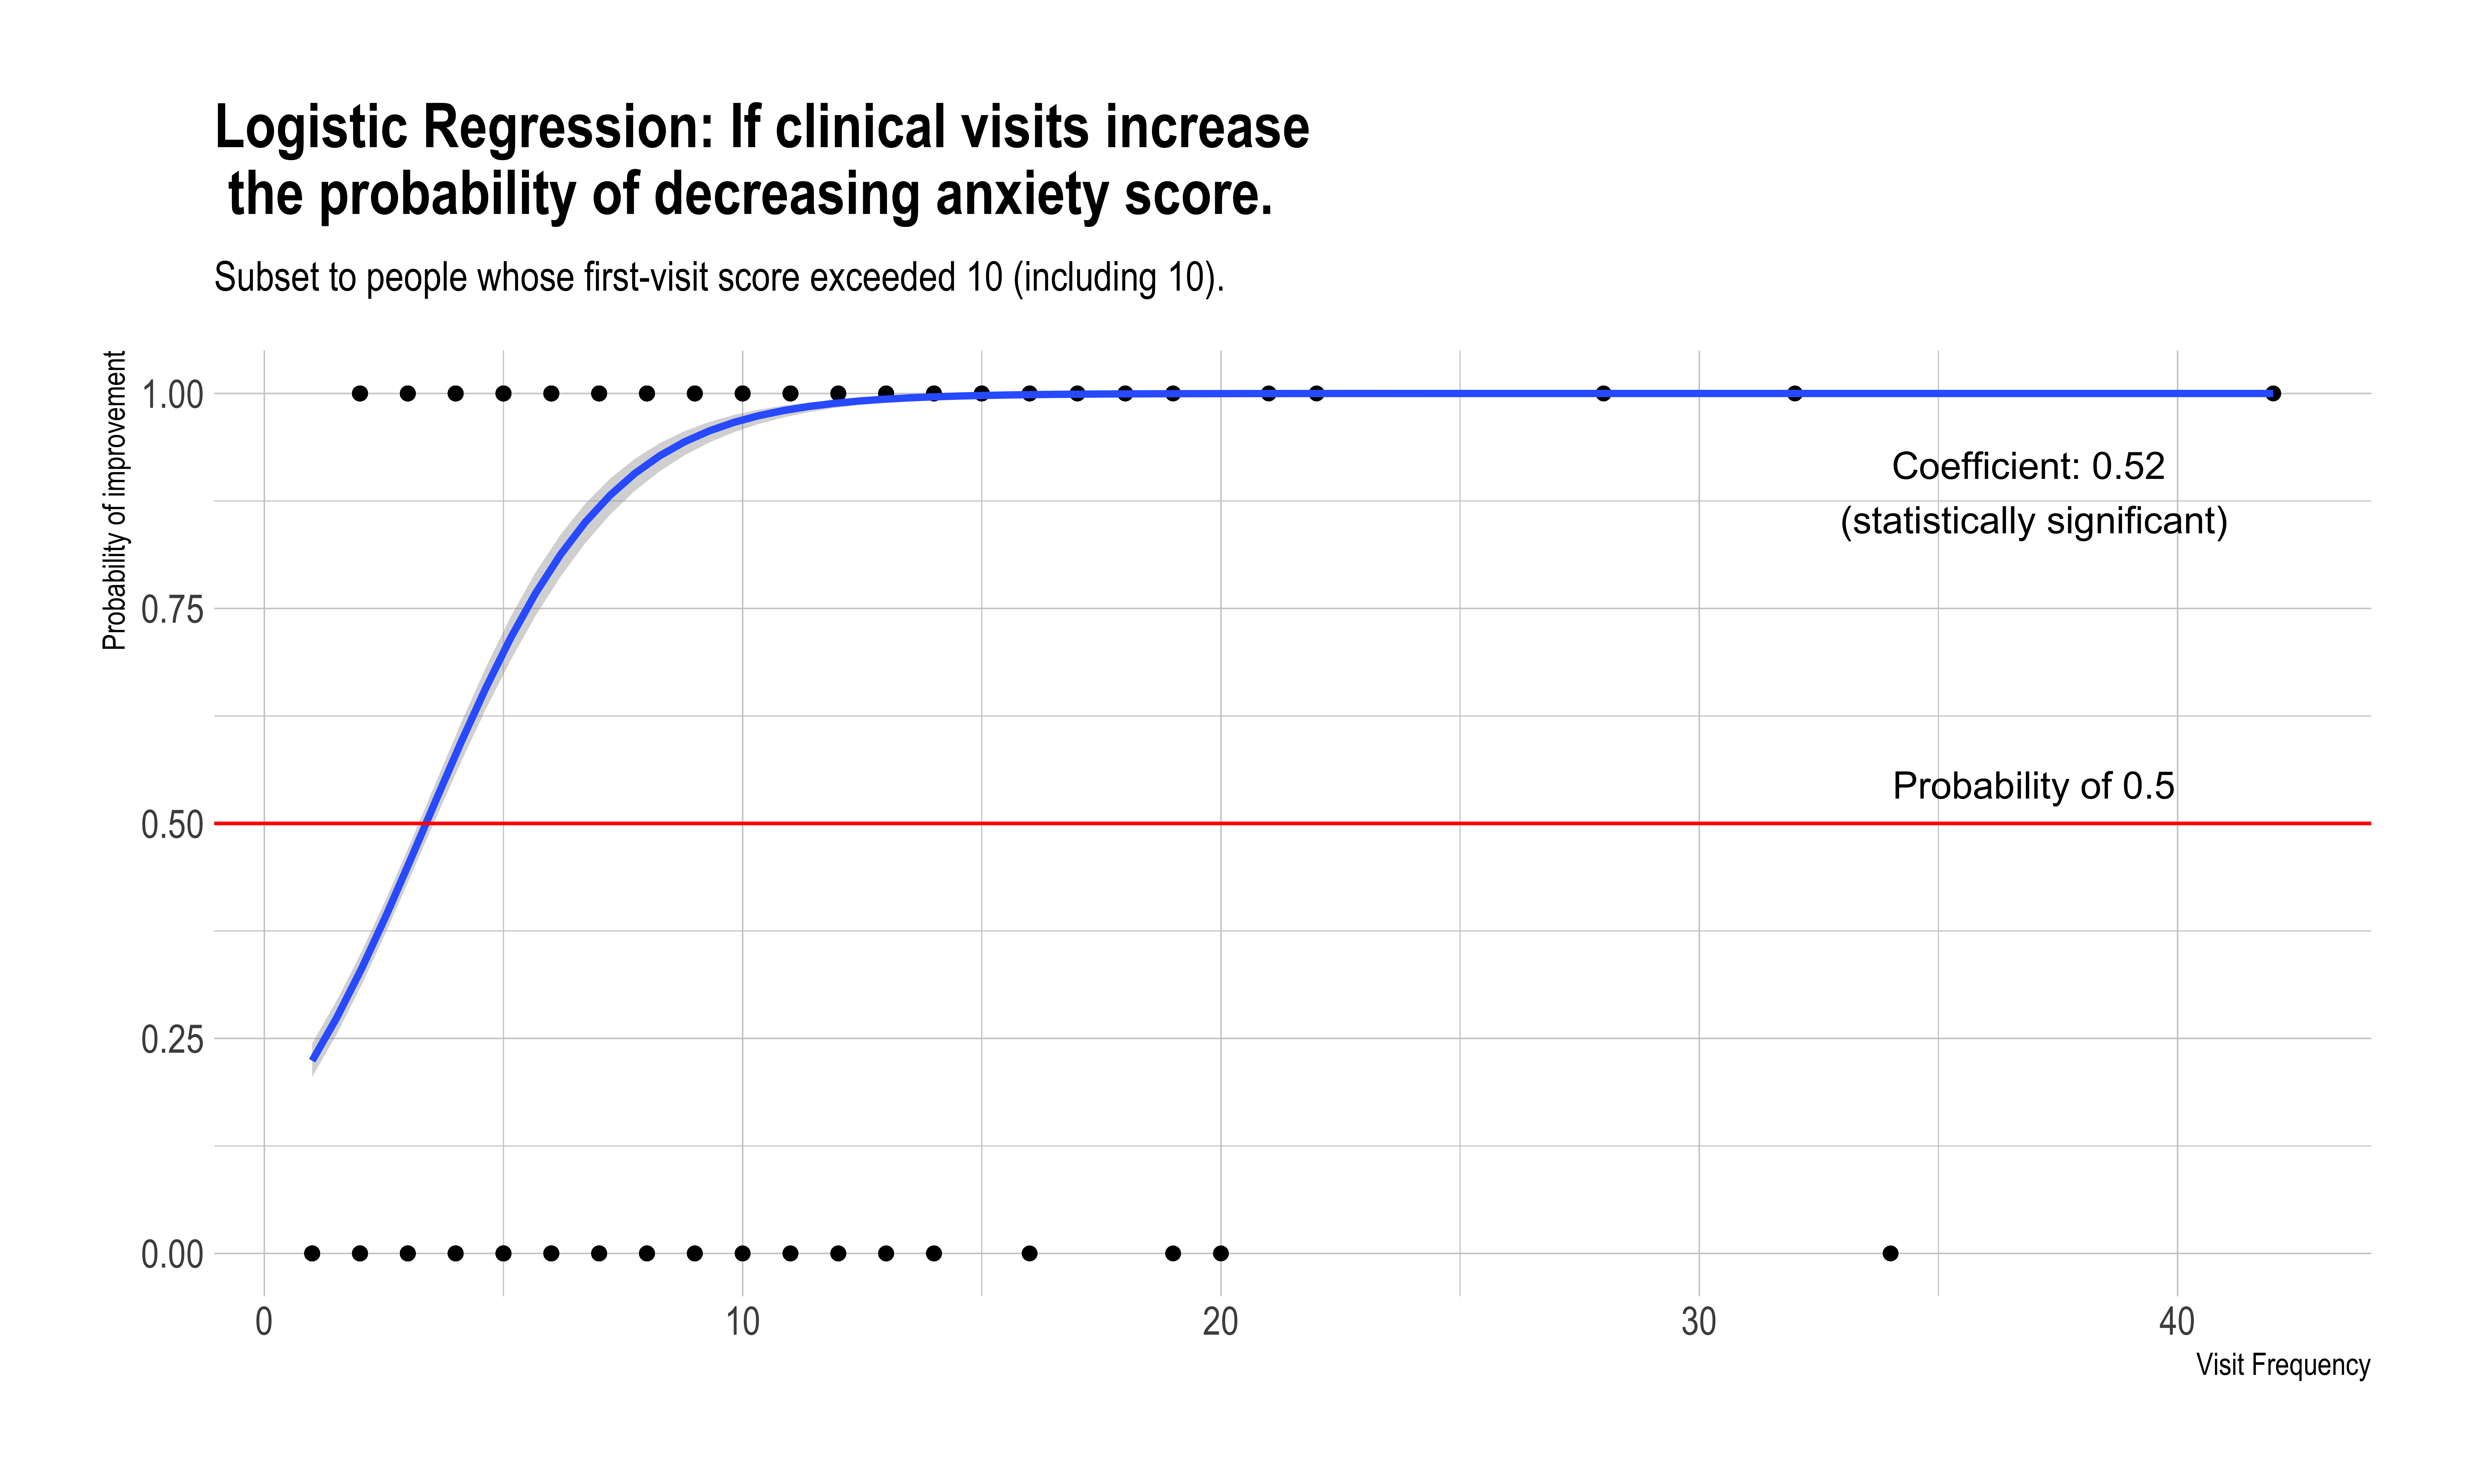
\includegraphics[width=\linewidth]{Figures/pp2.png}
			\caption{}\label{fig:pp2}
		\end{subfigure}
	\end{figure}

\end{enumerate}

\section{Discussion}

Evidences above all points to a positive effect of clinical treatment on patient's anxiety. But we definitely need to collect more data and information on more dimensions in order to provide better guidance or present stronger patterns to both mental health providers and patients. As can be easily imagined, anxiety level could be influenced by many factors such as internal personalities and characteristics, personal experiences, outside events, and even weather or geolocation. It is hard and implausible to exclude all these other influential factors in understanding and evaluating patients' anxiety score and further examine clinical treatment effect. I think there are some pieces of information that would be important to collect: 

\begin{itemize}
	\item \textbf{demographic variables}  such as age, sex, education background, work-status, marriage-status, wealth-condition, physical condition;
	\item \textbf{event variables} such as recent aquaintance, recent big event, anything that might wing his / her anxiety level greatly;
	\item \textbf{spatial variables} such as neighborhood information.
\end{itemize}
	
Based on the variables already available in our dataset, we can investigate a little the possible effects these other factors might have. Firstly, I wanted to check if testing in the morning or in the afternoon makes any difference in patients' anxiety level. Based on the date the measurement was made, I added a variable indicating whether it's am or pm. Figure \ref{fig:picture6} shows a strong pattern that generally speaking, patients tend to have higher anxiety level in the morning. Also, scores in the afternoon are less spreaded, which might signal a more stable anxiety level in the afternoon compared to the morning.

 \begin{figure}[htb!]
	\caption{Box plots comparing anxiety scores in am. VS. pm.}\label{fig:picture6}
	\begin{subfigure}[h]{0.48\linewidth}
		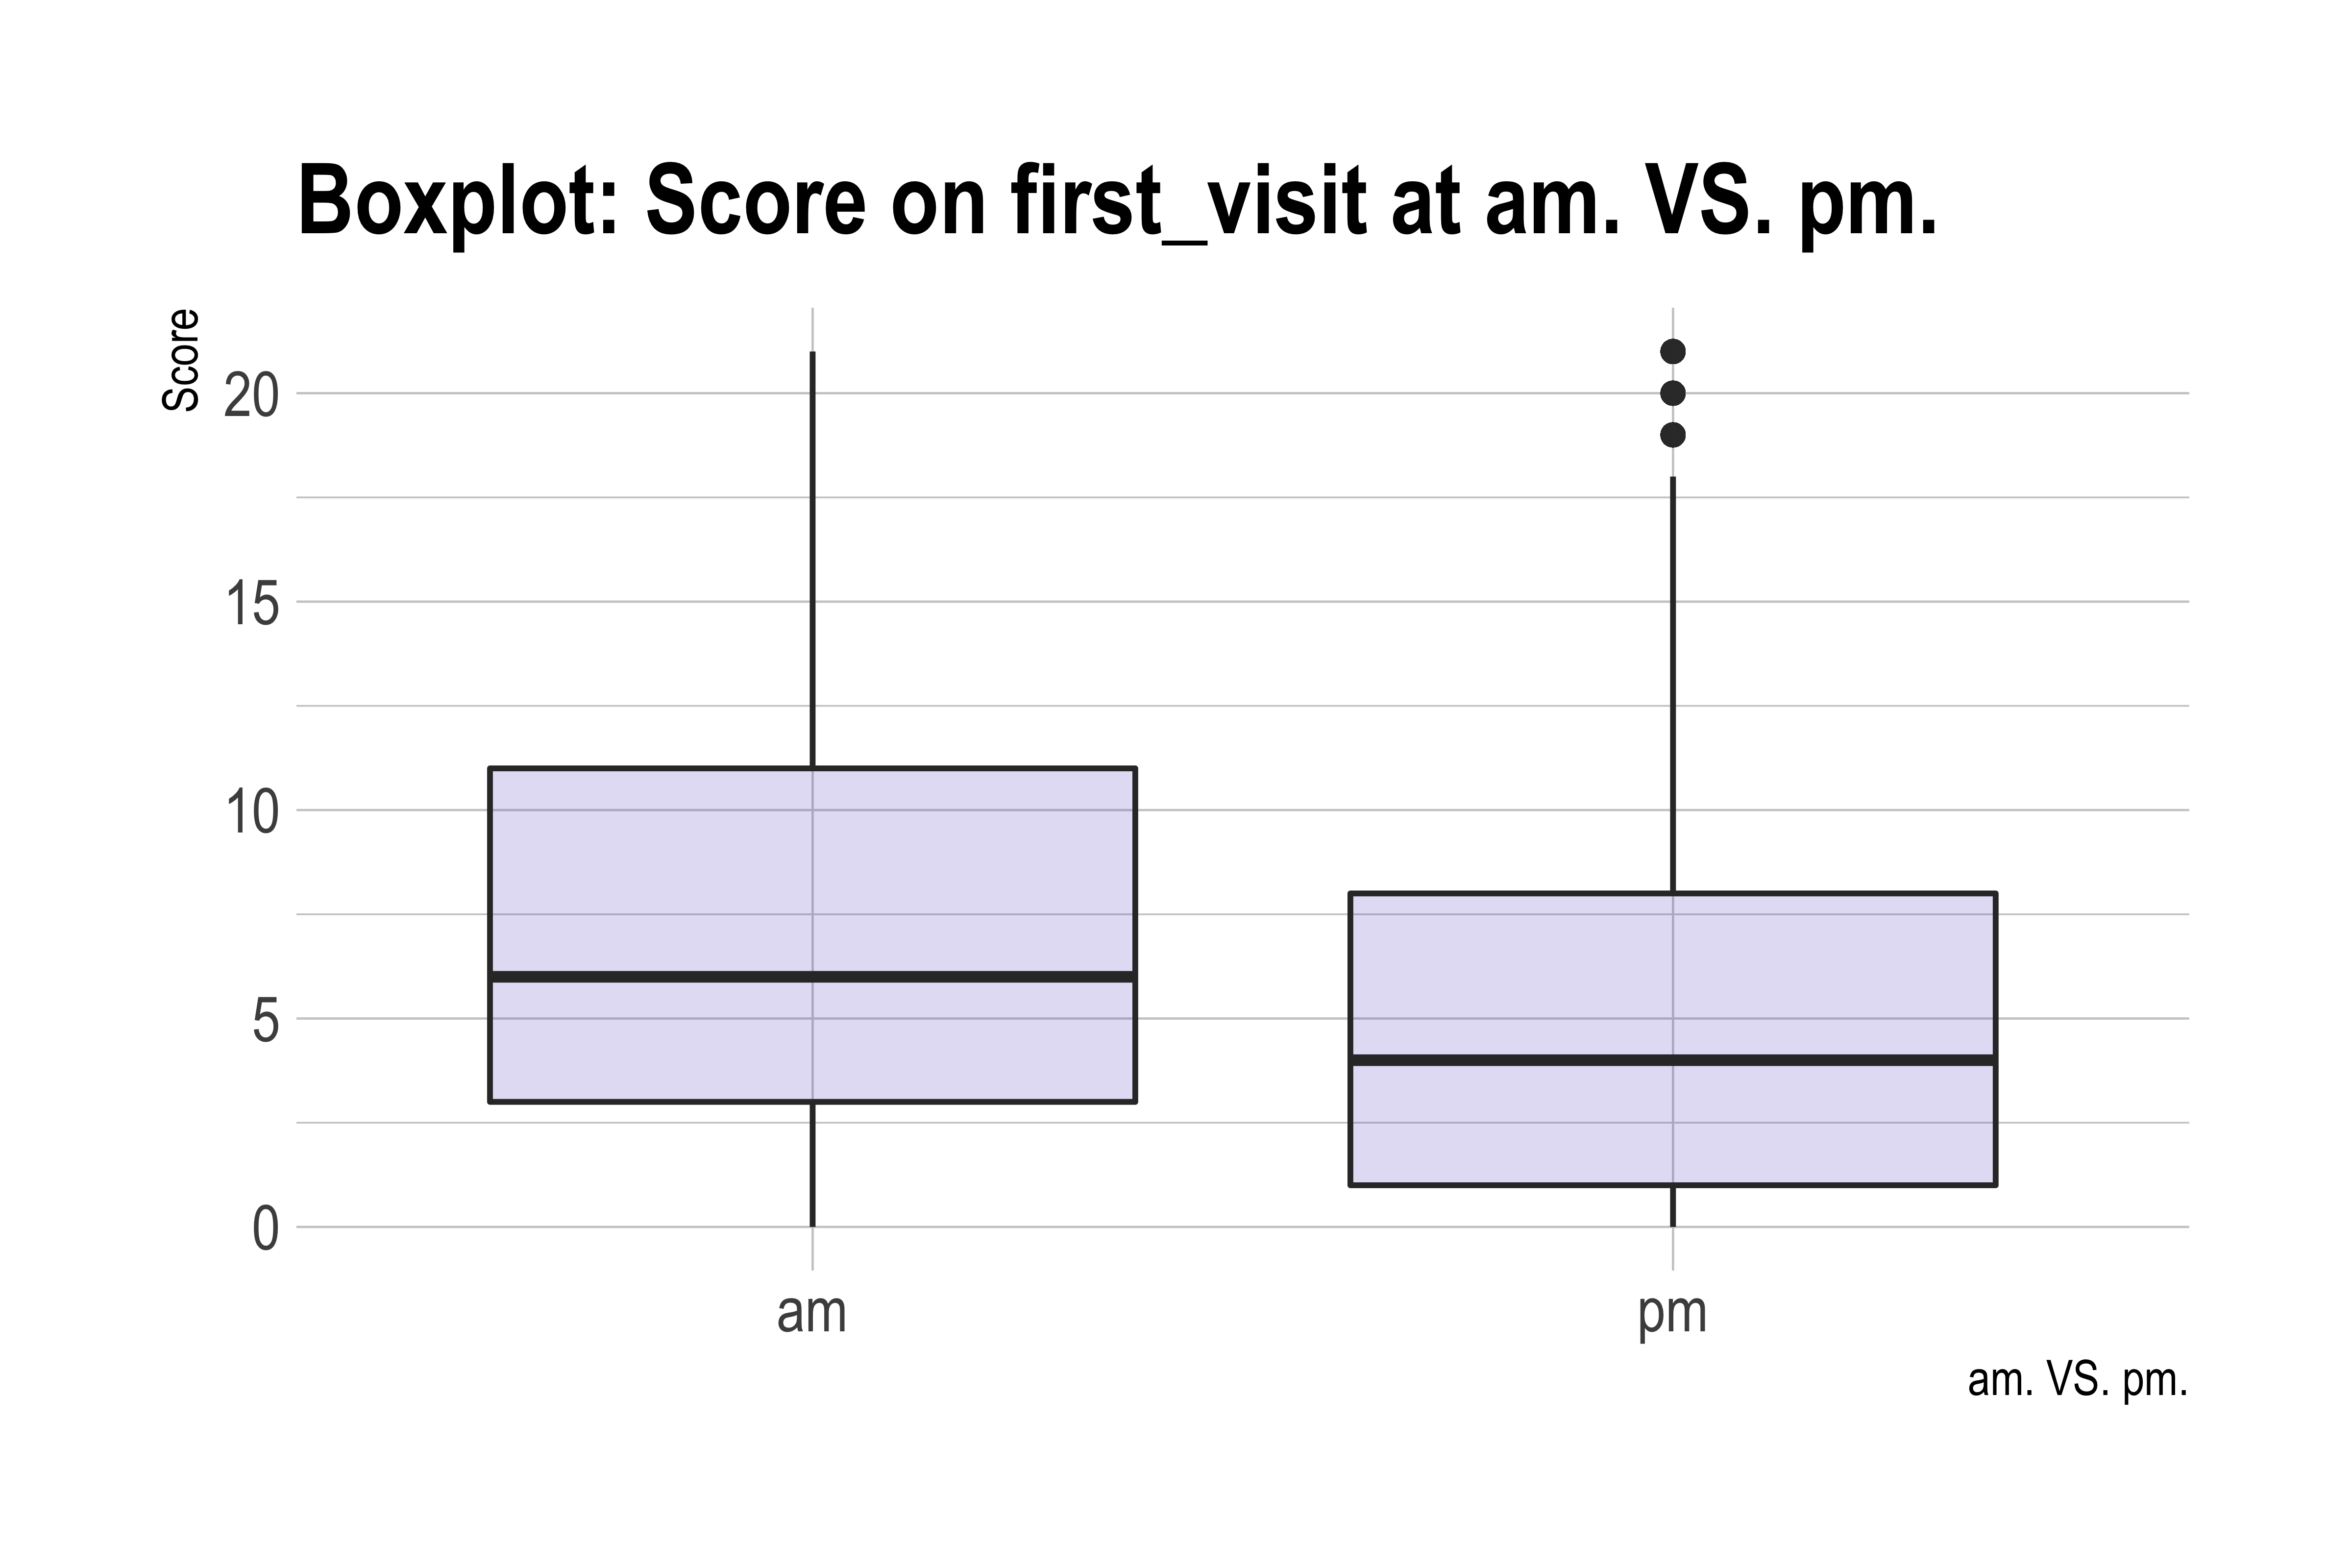
\includegraphics[width=\linewidth]{Figures/ppp1.png}
		\caption{}\label{fig:ppp1}
	\end{subfigure}
	\hfill
	\begin{subfigure}[h]{0.48\linewidth}
		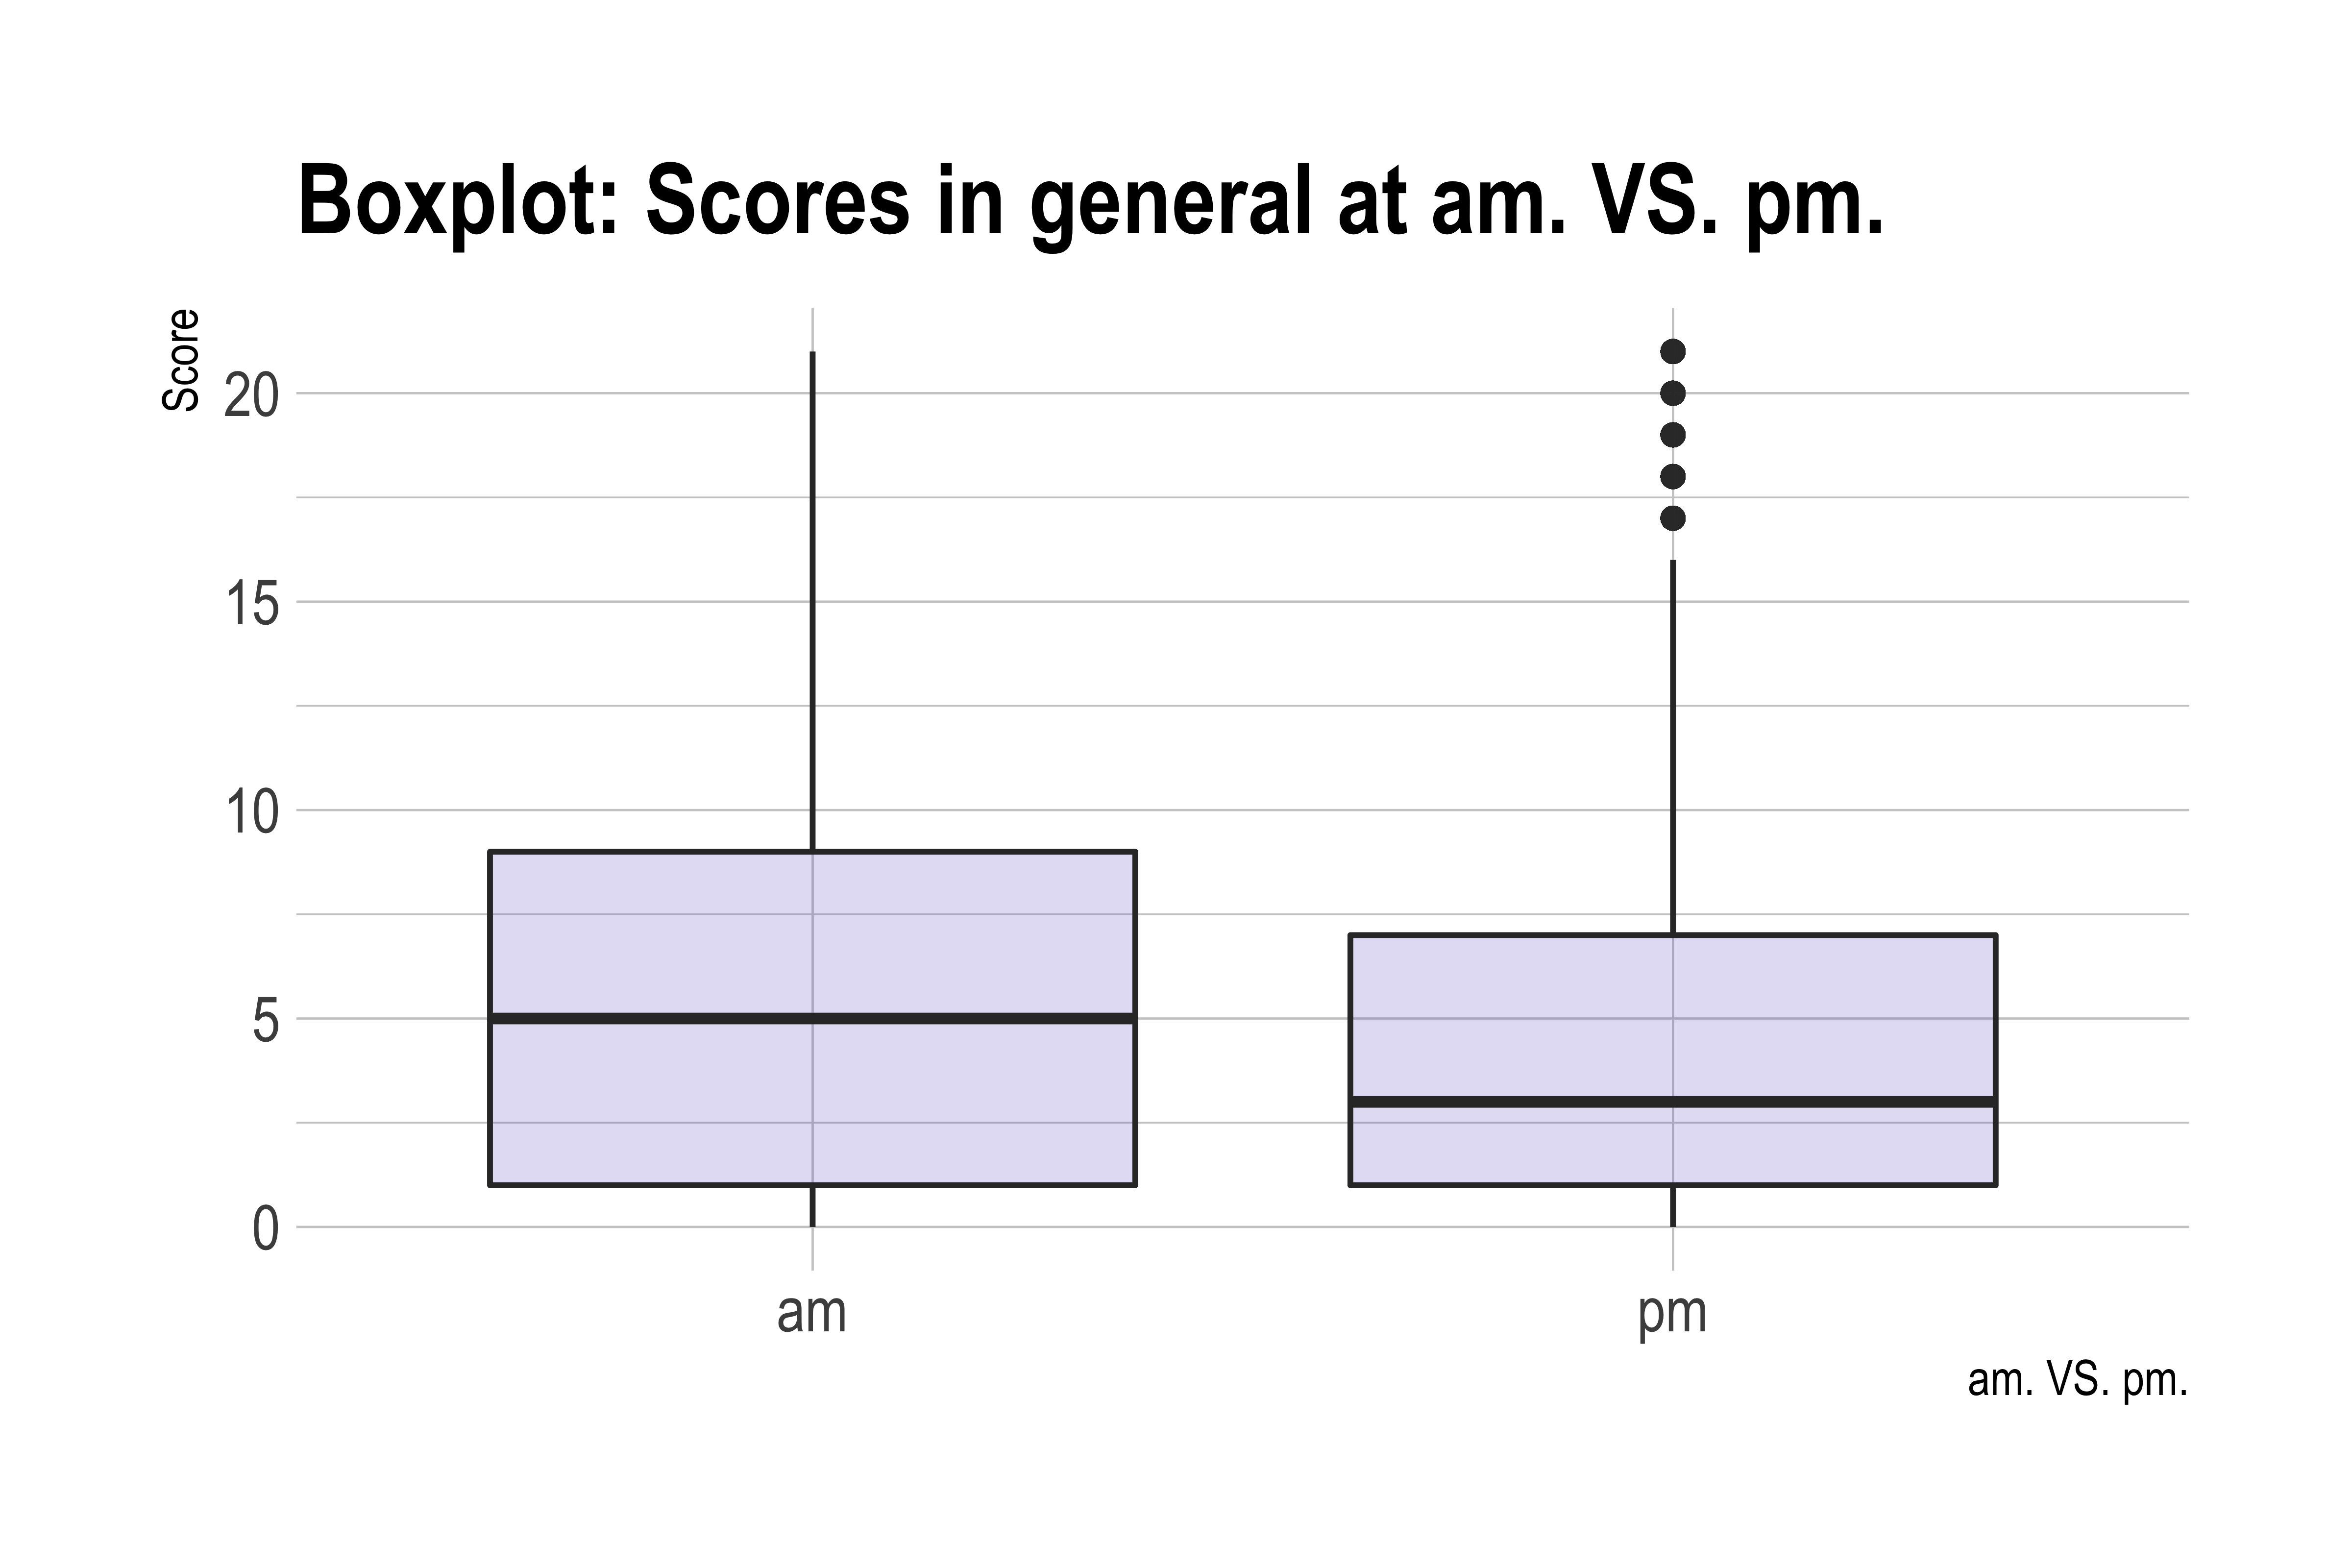
\includegraphics[width=\linewidth]{Figures/ppp2.png}
		\caption{}\label{fig:ppp2}
	\end{subfigure}
\end{figure}

Secondly, I plotted the time trends of anxiety scores for all patients (figure \ref{fig:picture7}) as well as only for patients with larger initial anxiety scores (figure \ref{fig:picture8}). I wanted to see if there's common trigger of any anxiety changes. We can see from figure \ref{fig:picture7} that the there is a clear trend of the overall anxiety level. 
% , which might be caused by the sudden lock-down or the rapidly increasing covid cases. Later on people seem to calm down a little and get used to the situation. 
However, by comparing figure \ref{fig:picture7} and figure \ref{fig:picture8}, we see that there seems to be no such trends for patients who already have a initial high anxiety level. This could suggest that many people that do not have high anxiety level are more badly influenced by covid wheras people that already have anxiety troubles did not get worsen. But we will need data from a longer time span both before and after covid for this statement.

\begin{figure}[htb!]
	\caption{Time trends}\label{fig:picture7}
	\begin{subfigure}[h]{0.48\linewidth}
		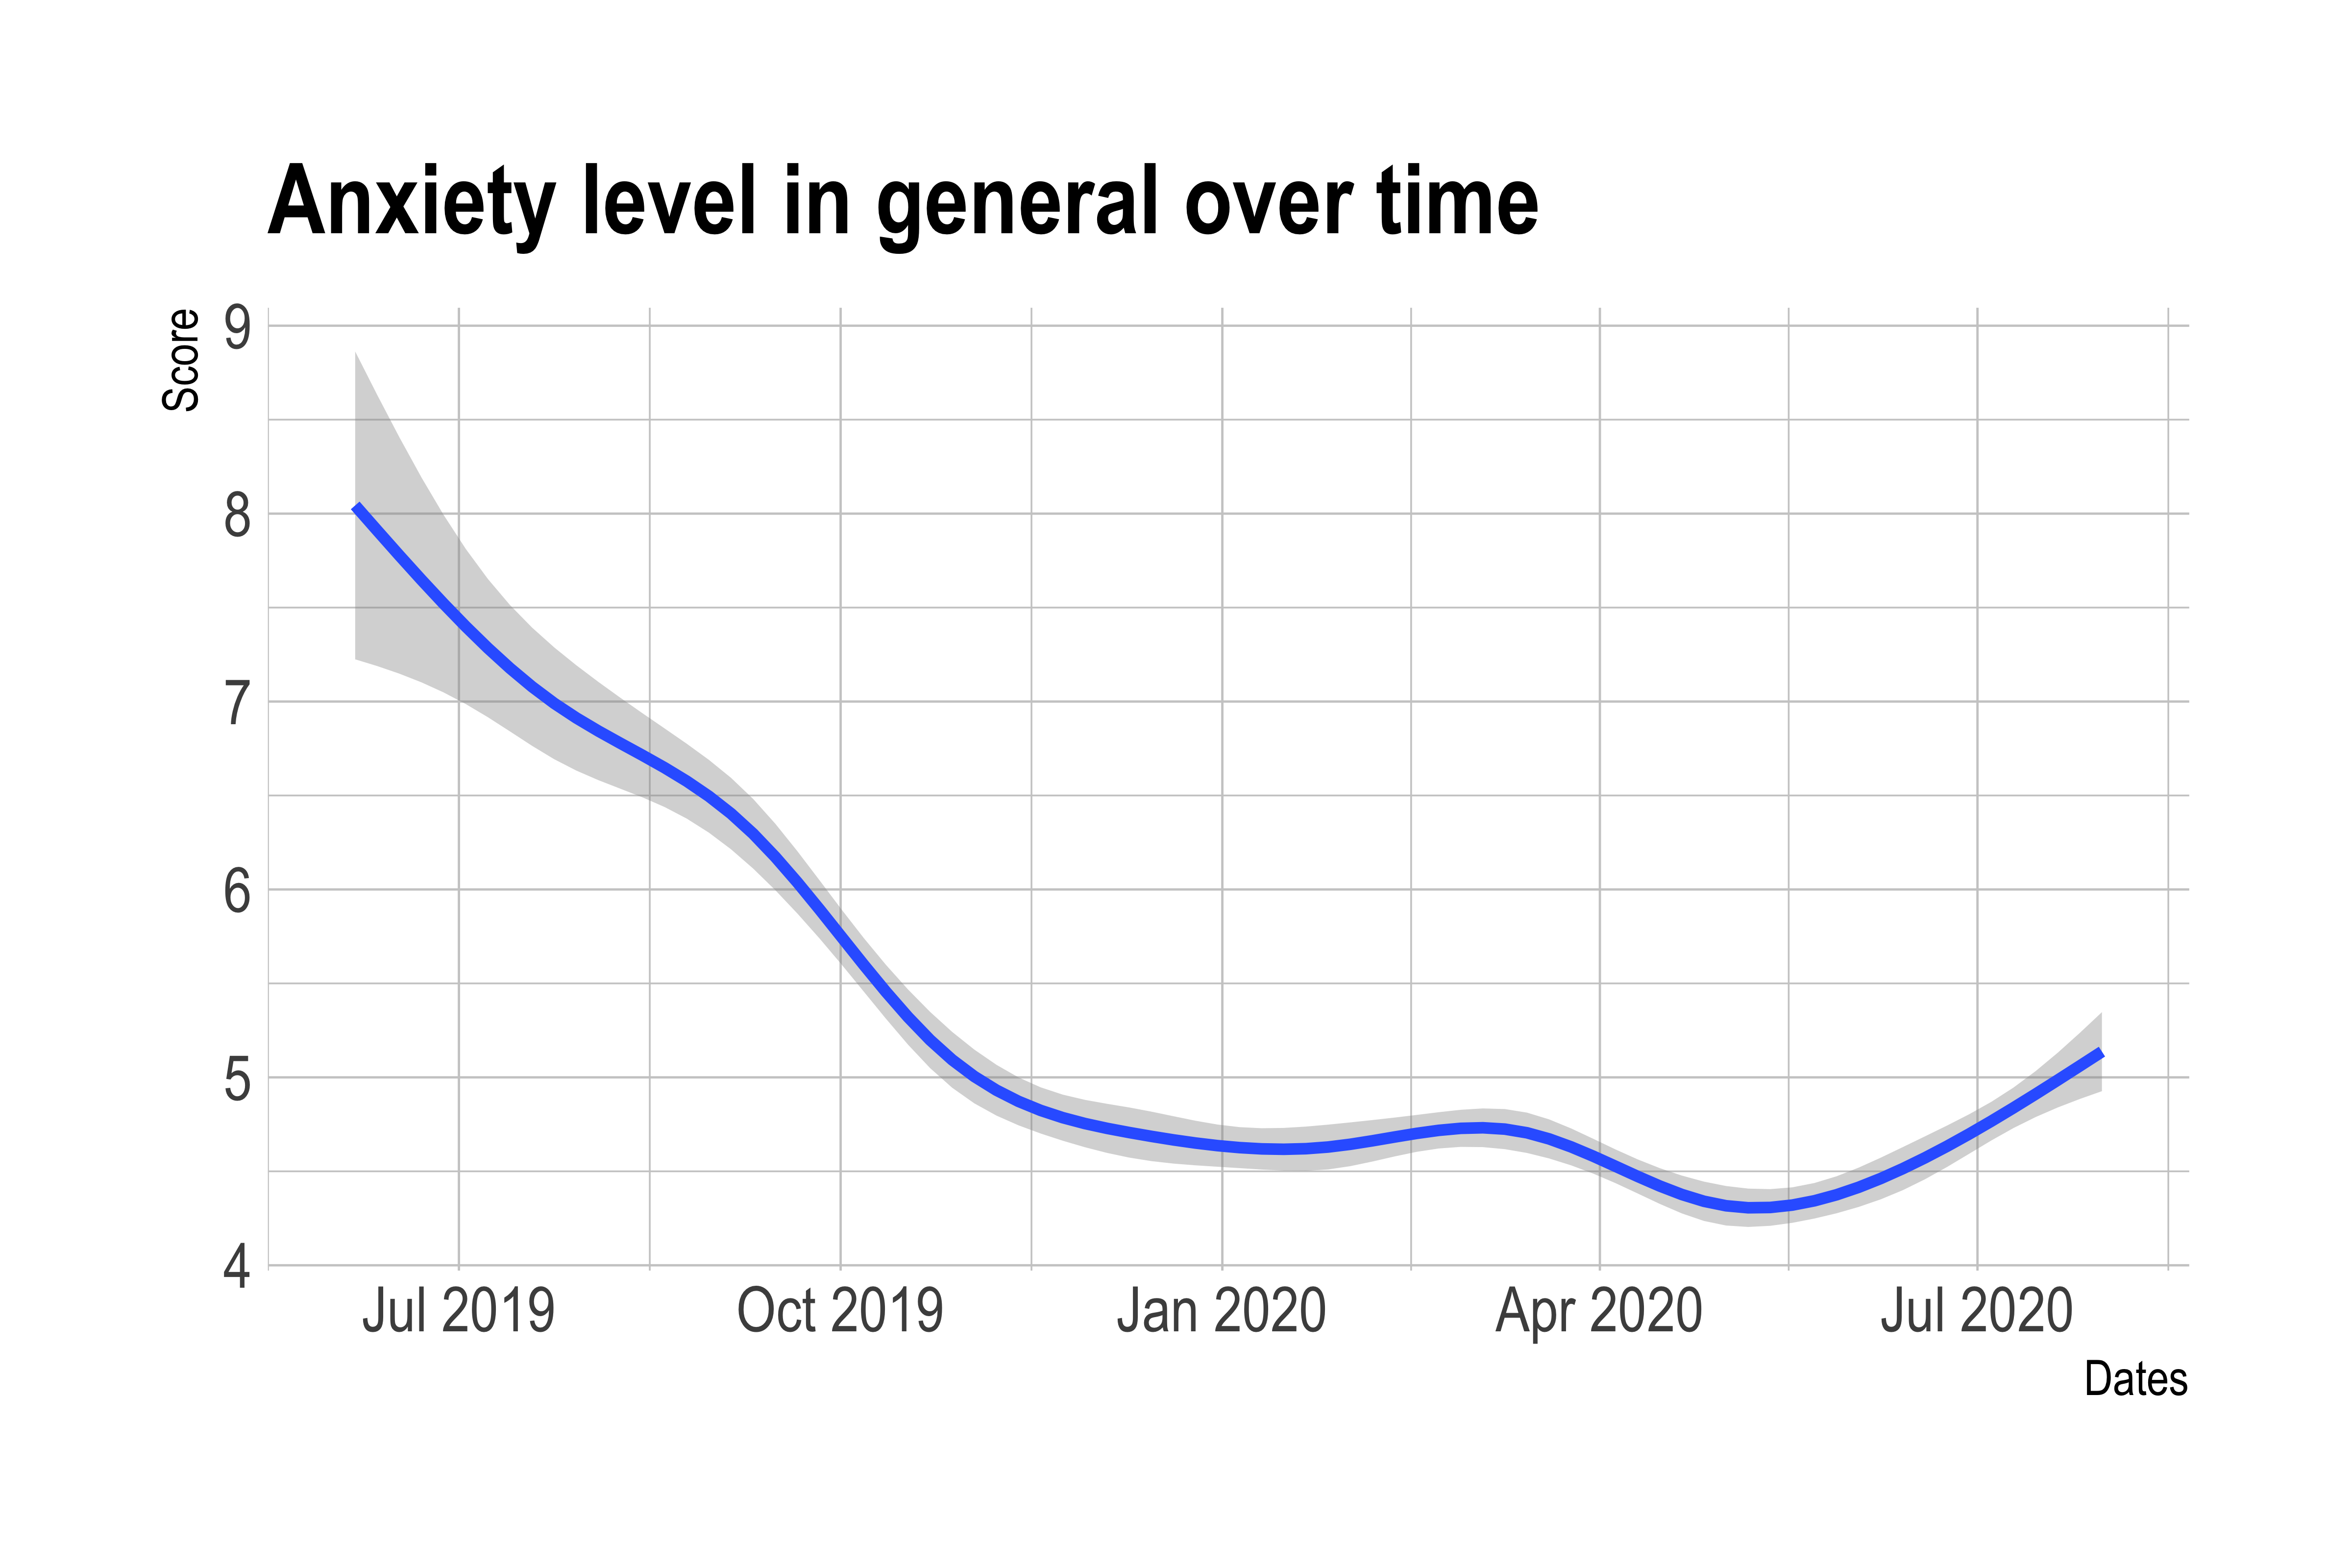
\includegraphics[width=\linewidth]{Figures/ppp3.png}
		\caption{}\label{fig:ppp3}
	\end{subfigure}
	\hfill
	\begin{subfigure}[h]{0.48\linewidth}
		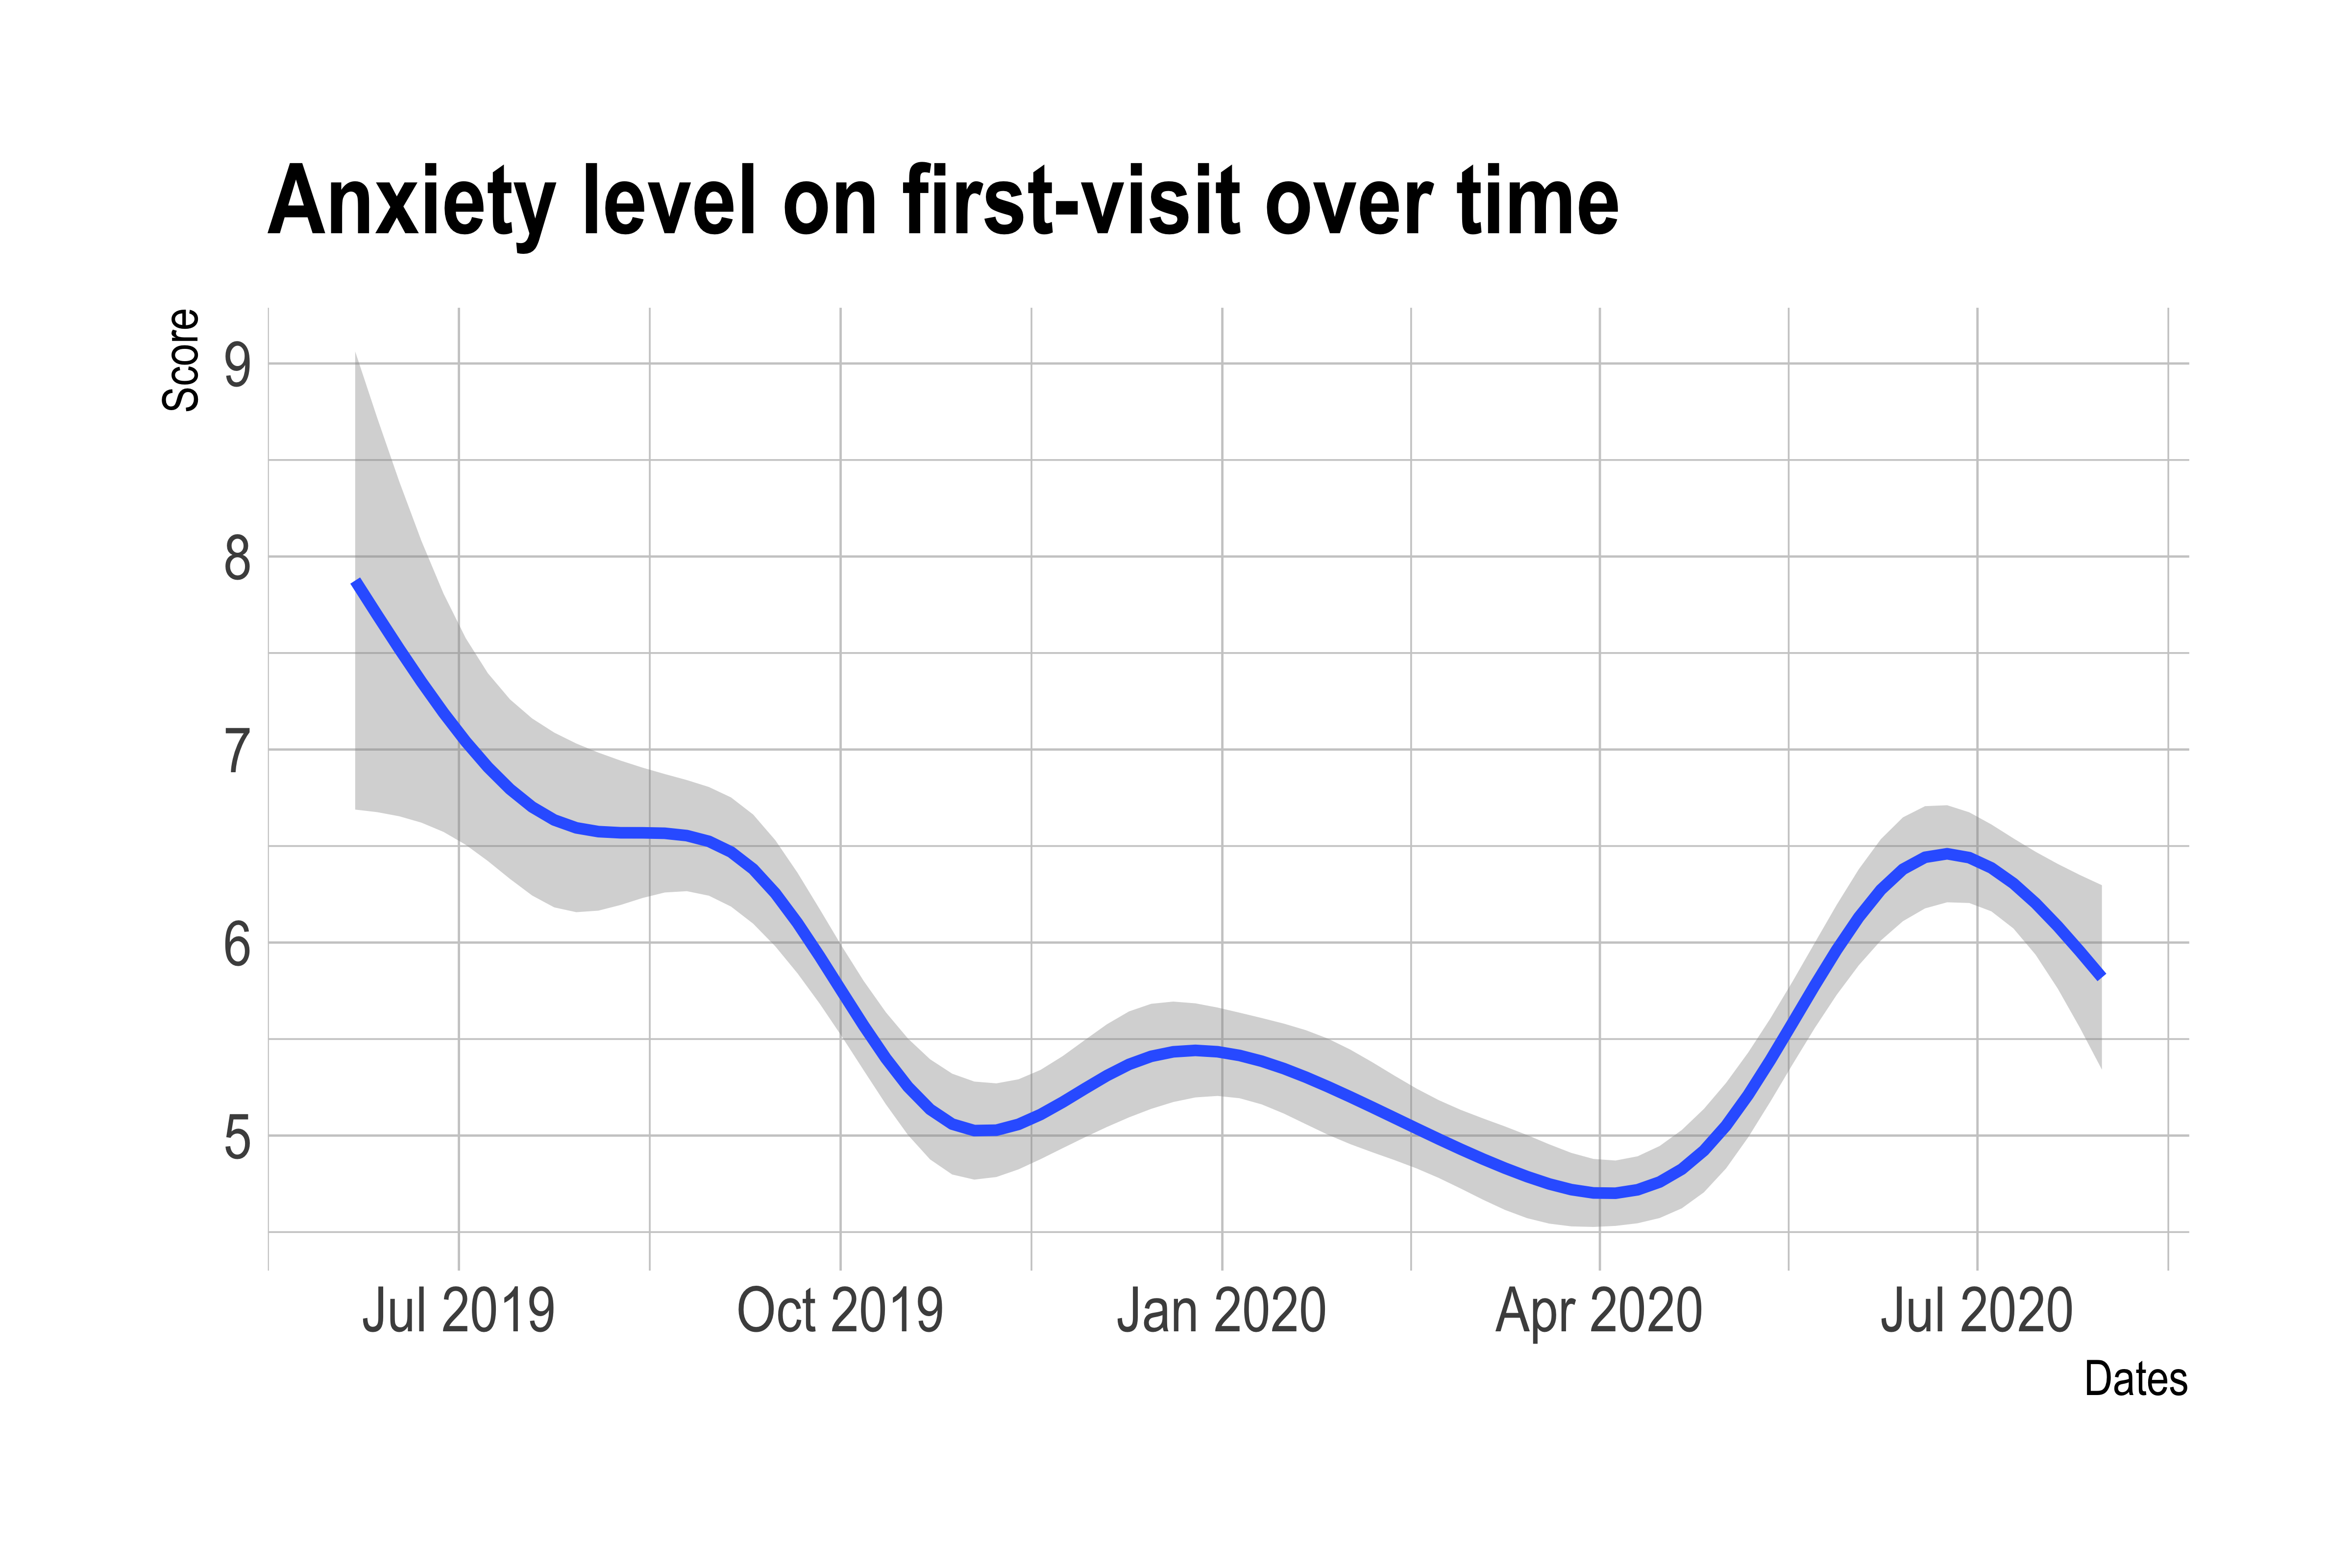
\includegraphics[width=\linewidth]{Figures/ppp4.png}
		\caption{}\label{fig:ppp4}
	\end{subfigure}
\end{figure}

\begin{figure}[htb!]
	\caption{Time trends}\label{fig:picture8}
	\begin{subfigure}[h]{0.48\linewidth}
		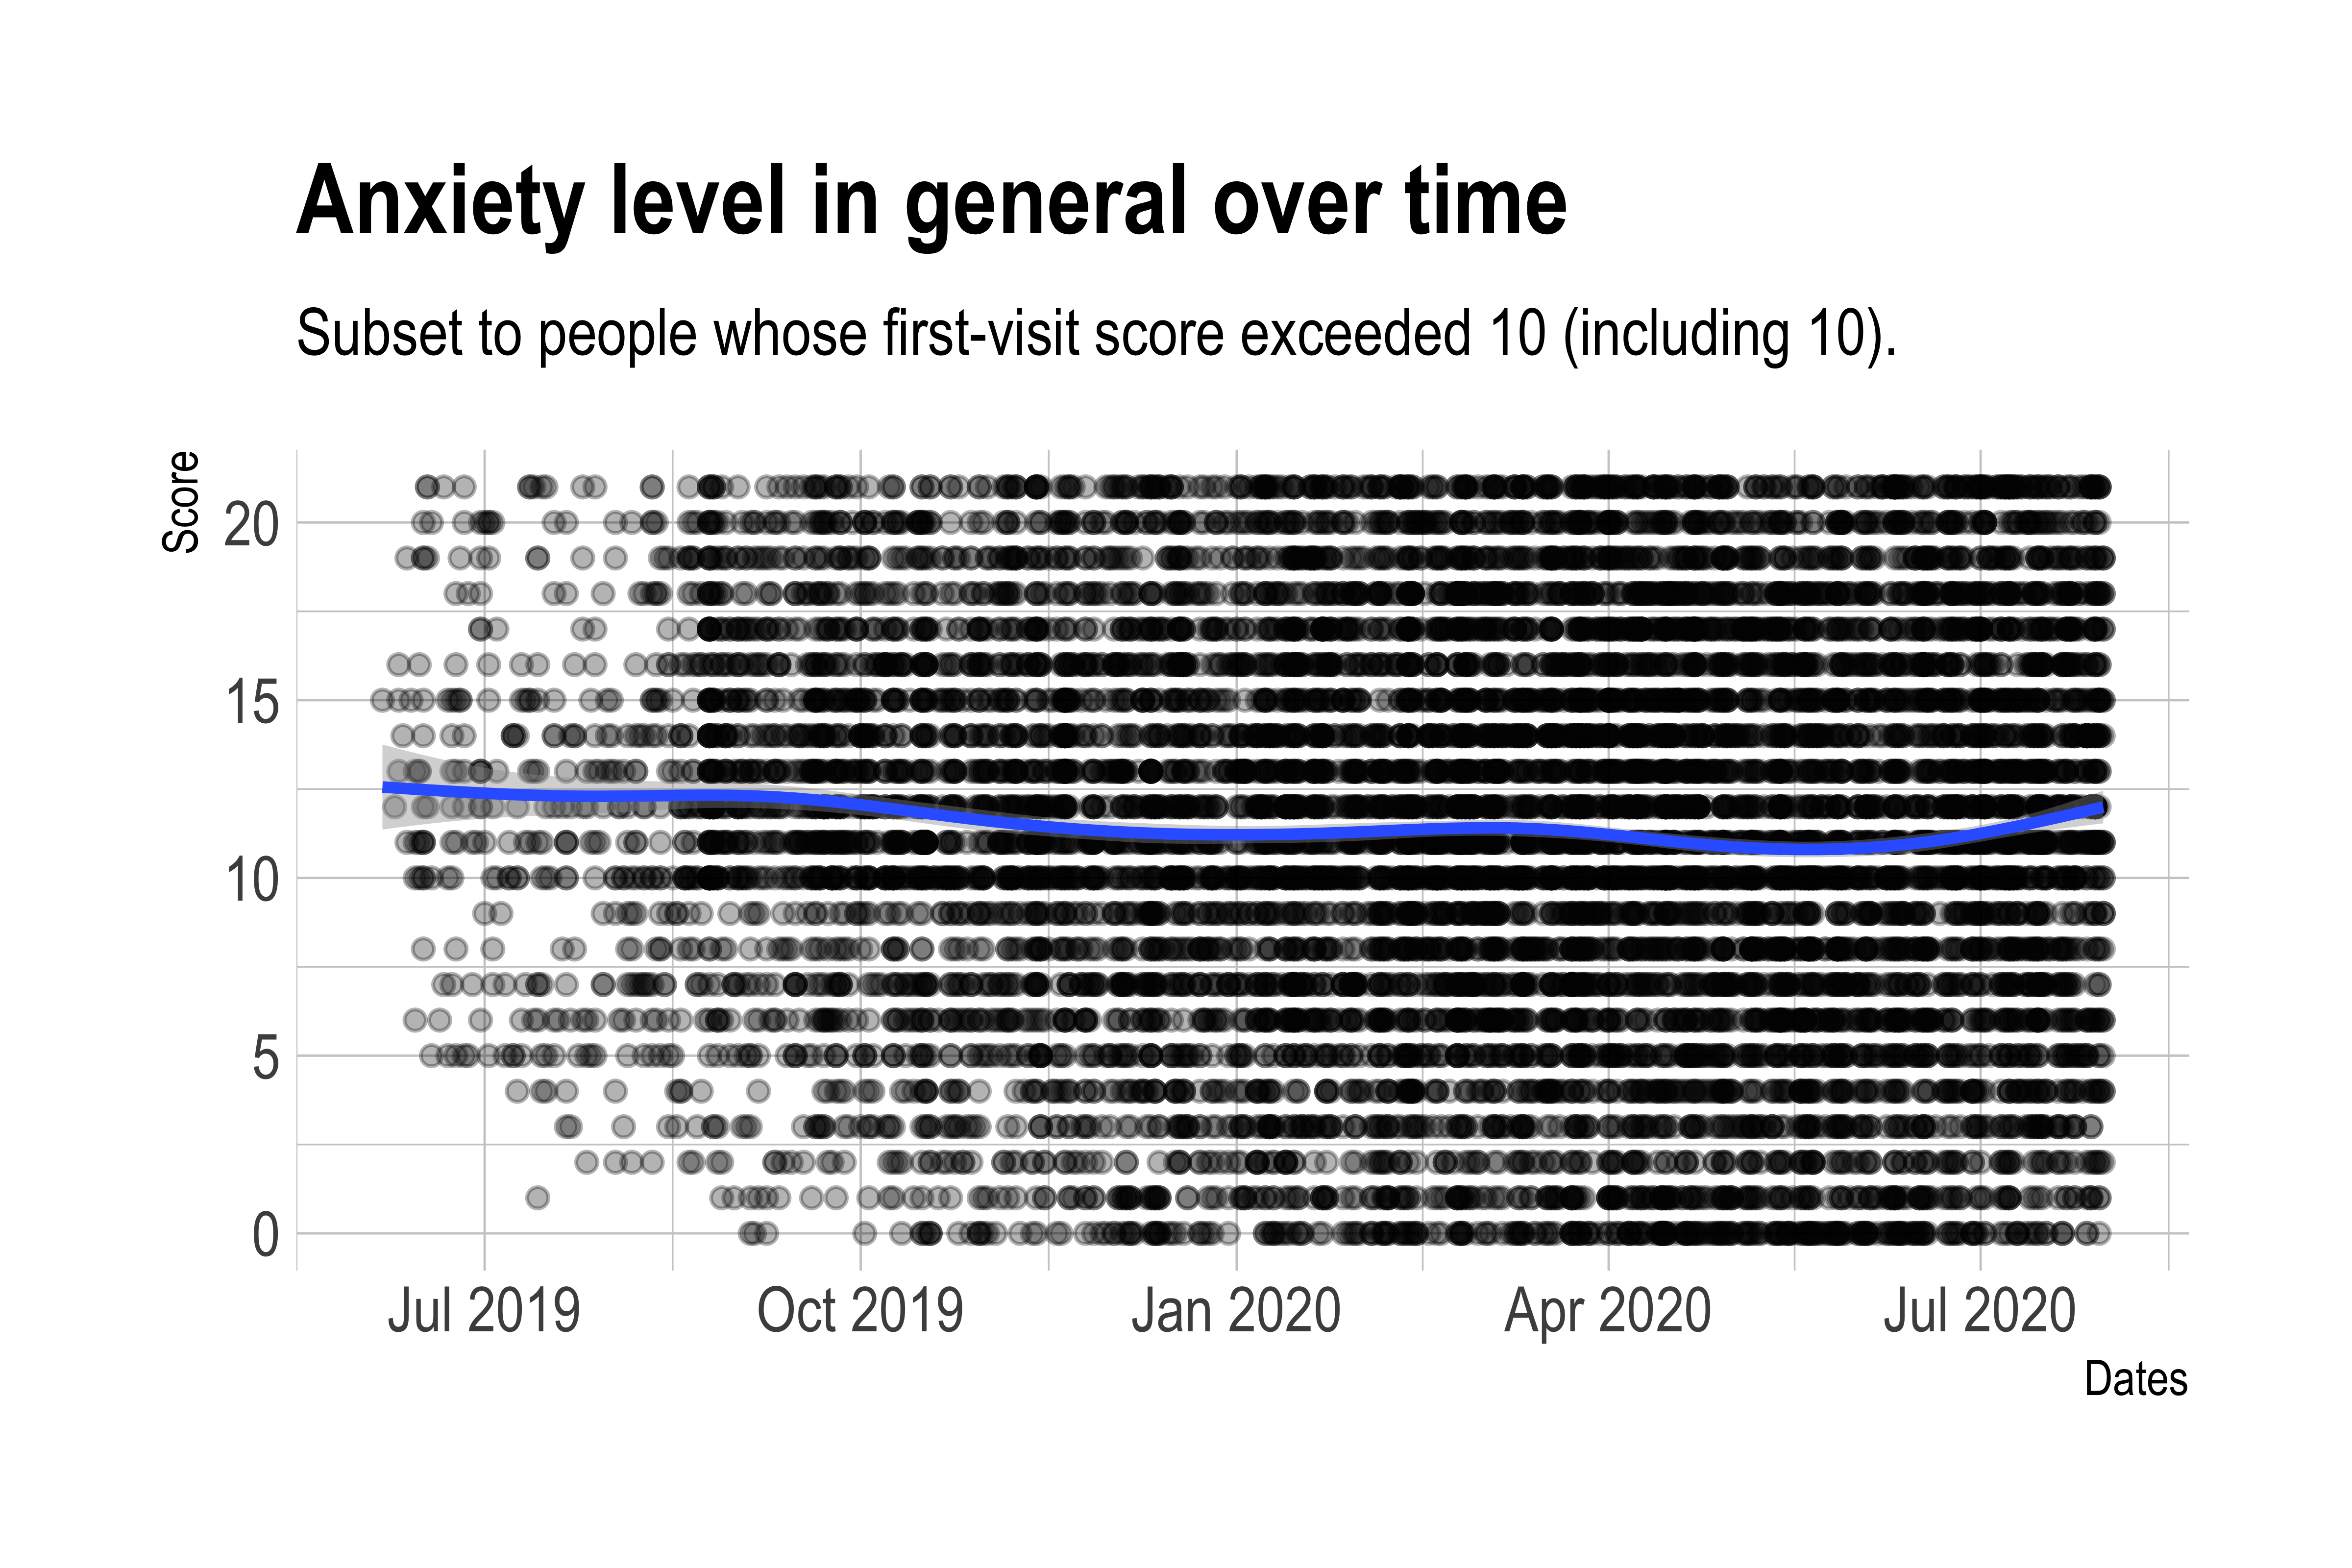
\includegraphics[width=\linewidth]{Figures/ppp5.png}
		\caption{}\label{fig:ppp5}
	\end{subfigure}
	\hfill
	\begin{subfigure}[h]{0.48\linewidth}
		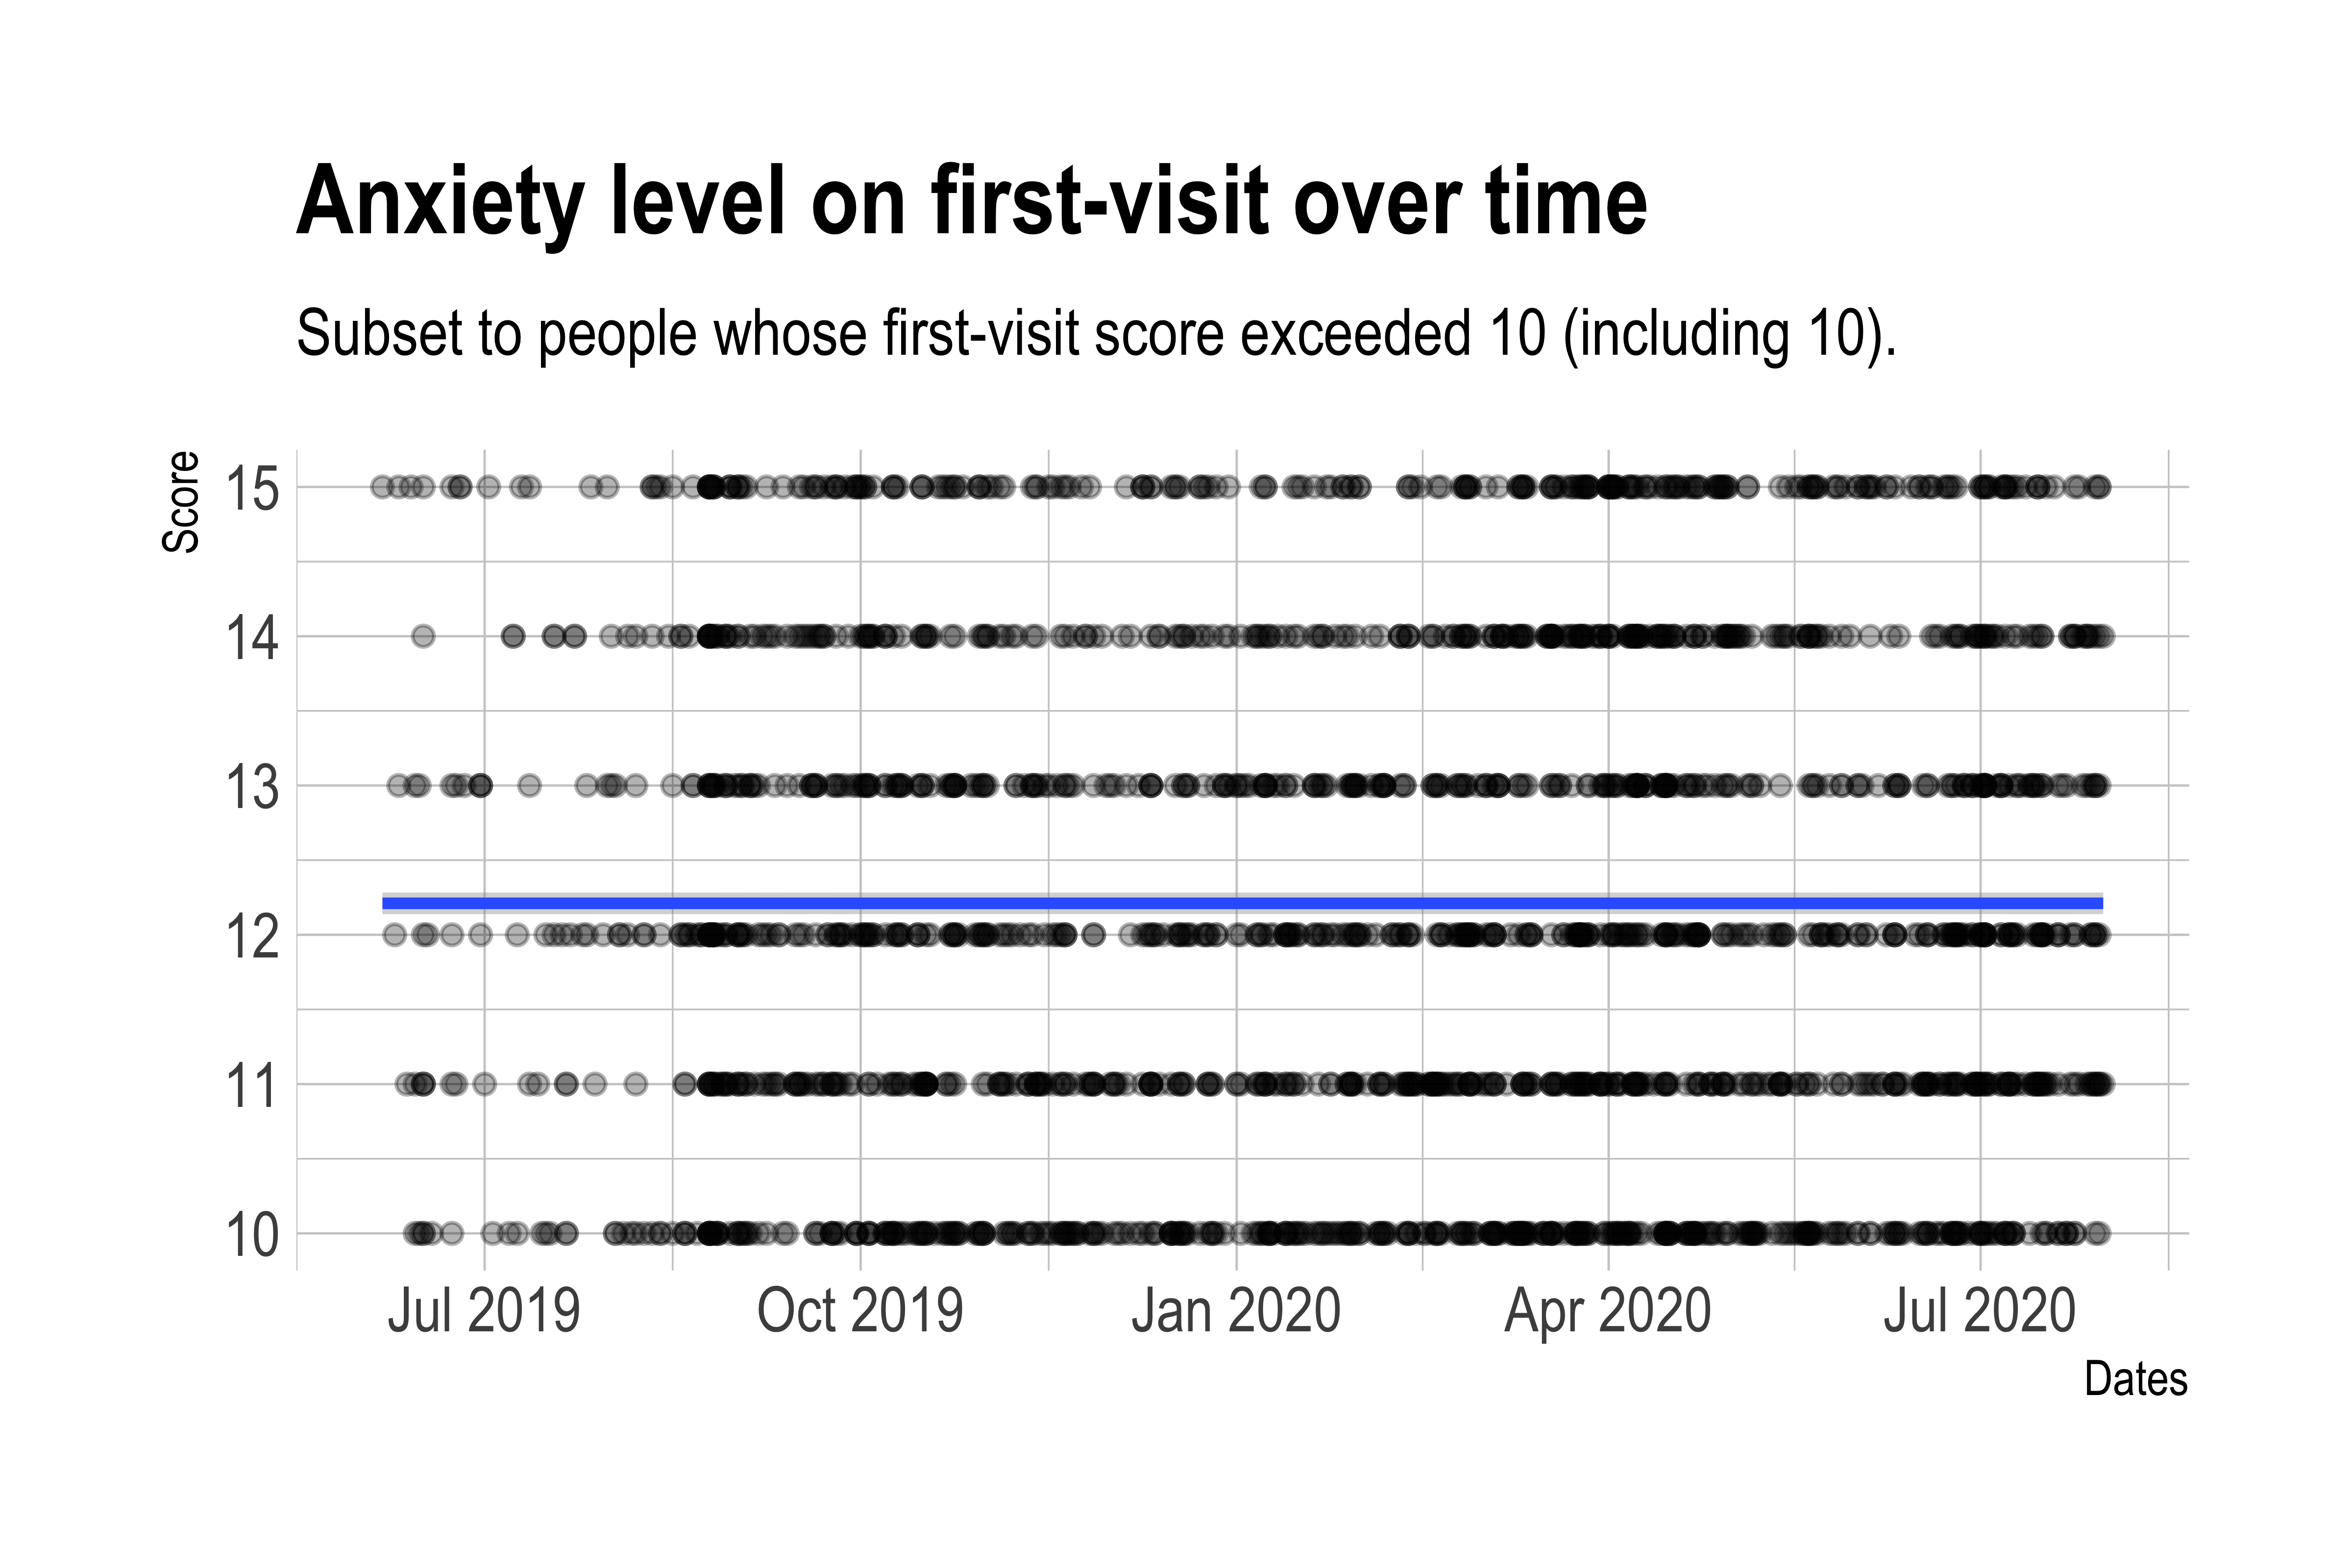
\includegraphics[width=\linewidth]{Figures/ppp6.png}
		\caption{}\label{fig:ppp6}
	\end{subfigure}
\end{figure}

	
\clearpage 

\end{document}
